\documentclass[12pt,oneside,openany,a4paper,%..... Layout
               afrikaans, english,%.............. Global language selection
               ]{memoir}

 \usepackage[masters-t,%.......................... Master thesis
             goldenblock,%........................ A5 type block (or a5block or wide)
            ]{usthesis}%.......................... US thesis style with memoir

%
% PLEASE read the USthesis documentation for the class options
% and how to set line and paragraph spacing
%

%==== Language setup ================================================
 \usepackage[latin1]{inputenc}%................... Recognizes �, �, etc
 \usepackage{babel}%.............................. Language setup

%==== Math setup ====================================================
 \usepackage{amsmath}%............................ Advanced math (before fonts)
 \usepackage{wasysym}
 \usepackage{siunitx}
 %\usepackage{amssymb}%............................AMS Symbol fonts

%==== Font setup (default is Computer Modern) =======================
 \usepackage[T1]{fontenc}%........................ Type 1 fonts
 \usepackage{textcomp}%........................... Additional text character
 \usepackage{bm}%................................. Bold math symbols (after fonts)

%==== Ref's, Bib's and Nomencl ======================================
 \usepackage{usnomencl}%.......................... List of symbols (in usthesis pack)
 %\usepackage[numbers]{natbib}%___________________ Vancouver style referencing
  
 \usepackage{usbib}%.............................. Bibliography    (in usthesis pack)
    \bibliographystyle{usmeg-a}
    %\bibliographystyle{IEEEtran}%________________ Arranging vancuver references numerically
    \renewcommand\bibfont{\small}
    
    

    %% For usmeg-a, the bib is a list of references. If you
    %% are using usmeg-n comment out the following lines
    \addto{\captionsafrikaans}{\renewcommand{\bibname}{Lys van Verwysings}}
    \addto{\captionsenglish}{\renewcommand{\bibname}{List of References}}

%==== Graphics and Color ============================================
\usepackage{graphicx}%........................... Graphicx loaded in usthesis
\usepackage{float}%___________Trying ti fix figure pos
\usepackage{color}%.............................. Color setup
\usepackage{eso-pic}%............................ Shipout commands for watermark
    \newcommand*{\WaterMark}[2][0.15\paperwidth]{%
        \AddToShipoutPicture*{\AtTextCenter{%
                \parbox[c]{0pt}{\makebox[0pt][c]{%
                    \includegraphics[width=#1]{#2}}}}}}


%==== Tables ========================================================
 \usepackage{array, booktabs, multirow} %%______________________________________ Tables
 \newcolumntype{P}[1]{>{\centering\arraybackslash}m{#1}}%___ Centering cell entries
 \newcolumntype{Q}[1]{>{\raggedright\arraybackslash}m{#1}}

 \newcommand{\tabitem}{~~\llap{\textbullet}~~}		%Bullets
 \usepackage{tabularx}		%Page width

 \usepackage[justification=centering]{caption}%_____________ Centering captions of tables and figures

%==== Other =======================================================
 \usepackage{csquotes} %____________________________________ Used for quotation marks


%==== Local Defs ====================================================
\makeatletter
% "to adjust category codes so as not to use \"
% Please insert user defined commands here
% and NOT in the document itself!
\makeatother

%==== TITLE PAGE ====================================================
\title{\bfseries
       \AorE{Monitering van kern temperatuur, hartklop, respiratoriese tempo, bloed suurstof versadiging en EEG deur middel van 'n draadlose oor probe\\[1ex]\normalfont\small\itshape(``Monitoring core temperature, heart rate, respiratory rate, blood oxygen saturation and electrical brain activity through a wireless ear probe'')
            }
            {Monitoring multiple medical signs through a wireless ear probe}
            }

\author{A.\ Bestbier}{Andr� Bestbier}

\degree{\AorE{MIng (Meg)}{MEng (Mech)}}
       {\AorE{Magister in Ingenieurswese (Meganiese)}
             {Master of Engineering (Mechanical)}}

\address{\AorE{%-- Afrikaans ----------------------------------------
        Departement Meganiese en Megatroniese Ingenieurswese,\\
        Universiteit van Stellenbosch,\\
        Privaatsak X1, Matieland 7602, Suid Afrika.%
             }{%-- English ------------------------------------------
        Department of Mechanical and Mechatronic Engineering,\\
        University of Stellenbosch,\\
        Private Bag X1, Matieland 7602, South Africa.
             }}

\faculty{\AorE{Fakulteit Ingenieurswese}%
              {Faculty of Engineering}}

\supervisor{Prof.\ PF.\ Fourie}

\setdate{9}{2017}

%\SetSponsor{The financial assistance of the National Research Foundation (NRF)
%    towards this research is hereby acknowledged. Opinions expressed and
%    conclusions arrived at, are those of the author and are not necessarily to
%    be attributed to the NRF.}


%====================================================================
%     MAIN DOCUMENT
%====================================================================
\maxsecnumdepth{subsubsection}
\maxtocdepth{subsection}

%\setcounter{tocdepth}{2}
%\setcounter{secnumdepth}{2}



\begin{document}

%==== Front matter ==================================================
 \frontmatter
 \WaterMark{UScrest-WM}
 \TitlePage

 \DeclarationDate{2017/09/09}
 \DeclarationPage

 \begin{abstract}[english]%===================================================
Add abstract.
\end{abstract}


\begin{abstract}[afrikaans]%=================================================
Voeg uittreksel by.
\end{abstract}


\chapter{Acknowledgements}%==================================================

I would like to express my sincere gratitude to the following people
and organisations ...


\chapter{Dedications}%=======================================================
 \vfill
 \begin{Afr}
 \begin{center}\itshape
    Hierdie tesis word opgedra aan ...
 \end{center}
 \end{Afr}
 \vfill
 \clearpage

%============================================================================
\endinput


 \tableofcontents
 
 \clearpage

 \setcounter{lofdepth}{2}
 \listoffigures
 \clearpage

 \listoftables
 \clearpage

 \chapter{Nomenclature}

\begin{Nomencl}
 \NomGroup{Constants}%-----------------------------------------------
   \item[$\mathrm{g} = $] $\mathrm{9.81\,m/s^2}$

 \NomGroup{Variables}%-----------------------------------------------
   \item[$\mathit{Re}_\mathrm{\,D}$]
                      \UnitLine{Reynolds number (diameter)}{~}
   \item[$x$]         \UnitLine{Coordinate                }{m}
   \item[$\ddot{x}$]  \UnitLine{Acceleration              }{m/s^2}\\
   \item[$\theta$]    \UnitLine{Rotation angle            }{rad}
   \item[$\tau$]      \UnitLine{Moment                    }{N{\cdot}m}

 \NomGroup{Vectors and Tensors}%-------------------------------------
   \item[$\overrightarrow{\bm{v}}$] Physical vector, see equation ...

 \NomGroup{Subscripts}%----------------------------------------------
   \item[$\mathrm{a}$] Adiabatic
   \item[$a$]          Coordinate
\end{Nomencl}



\endinput


%==== Main document =================================================
\mainmatter
   \setsecnumdepth{subsubsection}
%   \numberwithin{equation}{section}
%   \numberwithin{figure}{chapter}
%   \numberwithin{table}{chapter}

\chapter{Introduction}
\label{chp:Intro}
This thesis document reports on a project undertaken in die biomedical field of wearable electronics. Great advances in miniaturization of electronics and wireless communication have challenged and transformed the norm of the how we use electronics to listen to the language of our bodies: bio-signals.

The importance and usefulness of a continuous, wearable health monitor should not be underestimated. Access to accurate, long term data can lead to improved diagnosis of health issues and a better understanding of how our bodies react to drugs, exercise, emotions and the environment around us.

Traditionally, bio-signals monitoring is done with stationary equipment and with a dedicated device for each signal to be measured. It is easy to see that this is not suitable for continuous and mobile bio-signals monitoring. 

This project concerns the design, development and testing of a proof of concept device that will overcome the limitations of these traditional methods. The device is to be worn on the ear and will transmit its collected data through a wireless connection to a supporting system for storage and analysis.


\section{Aim/Research Question}
To develop and test a proof of concept of a wearable device that can monitor bio-signals and transmit collected data wirelessly to a warning and storage system. Bio-signals include core temperature, heart rate, respiratory rate, blood oxygen saturation and electrical brain activity.
Is the external ear canal a feasible location for the continuous monitoring of core temperature, heart rate, respiratory rate, blood oxygen saturation and electrical brain activity by means of a ear worn device?

In order to achieve the aim of of this project the following three objectives have to be met:
\begin{itemize}
\item Develop an ear worn device to measure core temperature, heart rate, respiratory rate, blood oxygen saturation and electrical brain activity through the external ear.
\item Conduct a trail to determine the functionality of this device.
\item Subsequently, evaluate the feasibility of an ear worm bio-signal monitor
\end{itemize}

\section{Motivation}
\chapter{Literature Review}
\label{chp:LitReview}
This chapter aims to describe the context within which the project is undertaken. The purpose of this literature review is to accumulate a thorough understanding of the current state of technology relevant to the project. Attention will be given to technical theory and work done by others in this field of research.

An overview will be given about the anatomy of the ear which is relevant to this study. Next, background will be given about each vital sign. Thereafter, the current technology available for monitoring vital signs will be reviewed.

\section{Ear Anatomy}
The area of the ear that is relevant to this study is the external ear. It includes the auricle, ear canal with surrounding tissue and the lateral side of the tympanum. This is the area available for the device to take the bio-signal measurement. Each part of the ear anatomy will be described, especially with regards to its ability to emit bio-signals or support the device in another way.

\subsection{Auricle}
The auricle is the visible part of the ear. It forms a C-shaped funnel that protrudes from the scull. Its structure is predominantly formed by yellow elastic cartilage covered in skin. Its complex folded shape differs from person to person, but certain structures are present in all normal auricles and have been named. As can be seen on Figure~\ref{fig:AuricleLabel} the concha is the indented part next to the ear canal. This area is an ideal location for a wearable device. The device can be held in place by the tragus and a probe can easily extend into the ear canal.

\begin{figure}
   \centering
   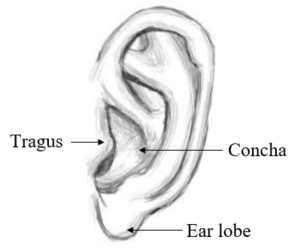
\includegraphics[scale=1]{figs/AuricleLabel}
   \caption{Drawing of the auricle (goo.gl/mmLnFx)}
   \label{fig:AuricleLabel}
\end{figure}

The external ear is supplied with blood from the auricular arteries. These arteries branch from the carotid artery which supplies the rest of the brain with blood. Being made mostly of cartilage and being at an extremity of the body, the auricle is not a suitable location for taking temperature measurements for its temperature is easily influenced by the ambient conditions.

The layer of skin covering the auricle contains blood vessels. It is possible to detect a pulse in the auricle, in fact, the ear lobe is a prime location for traditional pulse oximetry measurements. This is a possible location for a ear-worn device to make a heart rate measurement \citep{poh2010motion}. The ear lobe's blood vessels are, however, susceptible to vasoconstriction due to cold or hypovolaemia \citep{WHO2011UsingPulseOxi}. This will make is harder to get accurate heart rate measurements.

The auricle is used in EEG systems as a location for a reference electrode. It is far enough from the brain for it to have an extremely small electrical potential \citep{nunez2006electric}. More will be said about EEG referencing in Section \ref{}

\subsection{Ear Canal}
The external ear canal is the tube running from the floor of the auricle to the middle ear, ending blindly at the tympanic membrane or tympanum. Figure~\ref{fig:EarSection} depicts the structure of the ear as seen from a coronal plane section.
 
\begin{figure}
   \centering
   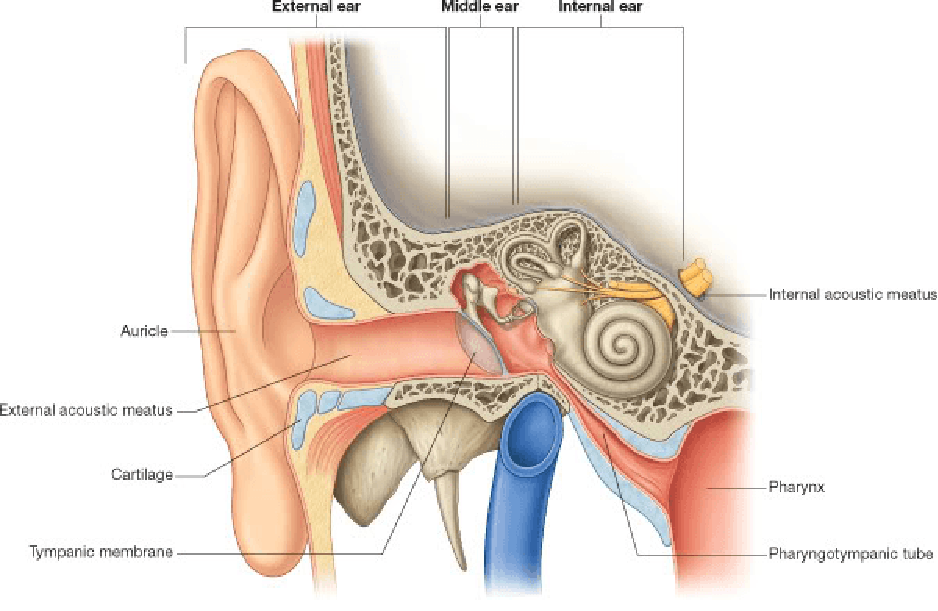
\includegraphics[scale=0.7]{figs/EarSection}
   \caption{Structure of the ear (Drake et al: Gray's Anatomy for Students)}
   \label{fig:EarSection}
\end{figure}
 
The ear canal in adults is approximately 25 mm long and have a diameter of 5 to 7 mm \citep{alvord1997anatomy}. The outer third of the external ear canal is surrounded by cartilage and fibrous tissue \citep{ExternalAuditoryCanal}. The inner two thirds are surrounded by the temporal bone. Thin skin from the lining of the canal and contains glands secreting ear wax. Hairs are found in the outer part of the canal. The ear canal of infants starts out relatively straight, but obtains a definite S-shape as the head develops \citep{alvord1997anatomy}. Ear canal shape varies from person to person. Therefore, an ear probe should be able to adjust to variation in ear canal shape and size.

The secluded nature of the ear canal means that it has a relative constant temperature. As with the auricle, the canal wall temperature will also be influenced by the ambient temperature, but to a much lesser extent. The wall of the ear canal is well supplied with blood. Blood vessels just beneath the thin layer of skin makes the ear canal a possible location for measuring heart rate and blood oxygen saturation. The ear canal extend toward the brain and electrical brain activity is present due to the conductive nature of the tissue. According to \cite{nunez2006electric} currents from brain potentials can be focused through holes in the scull, like the ear and nose. The farther away the origin of the signal is from the electrode, the weaker the measured signal will be. Therefore, an electrode in the ear canal will detect electrical brain activity near the ear better, including the temporal lobe and brain stem.

\subsection{Tympanum}
The tympanum forms the medial boundary of the external ear canal. It is a smooth elliptical membrane with a thickness of about 0.074 mm \citep{alvord1997anatomy}. The membrane is slanted with regards to the external ear canal. The tympanum is also supplied with blood from a branch of the carotid artery, therefore sharing its supply with the brain including the hypothalamus, the thermoregulation centre of the body. It is the most medial part of the external ear, and is therefore the least susceptible to influence by the ambient temperature. This is the reason that the tympanum is one of the best locations to measure core body temperature. The location is used by physicians to measure core temperature for it is quick and minimally invasive. Variations in body temp can be sensed faster on the tympanic membrane than on other locations on the body.  Contact with the tympanum can cause discomfort and harm to the patient, so non-contact infra-red thermometers are usually used.


\section{Bio-signal Physiology}
This section reviews the theory and research done about the physiological aspects of bio-signals. The origin and importance of measuring bio-signals will be discussed. This includes the typical readings expected from healthy adults, as well as the causes and implications of deviations from these healthy bio-signals.

The body constantly strives to maintain its internal environment at a stable state, suitable for its various physiological processes. Deviations from this stable state...

\subsection{Core Temperature}
Thermoregulation is the body's way of keeping its internal temperature within certain bounds to create a favourable environment for chemical reactions to take place. The temperature control centre of the body is in the hypothalamus and it regulates temperature by maintaining a fine balance between heat production and heat loss. Normal human core temperature varies between $36.5^{\circ}C$ and $37.5^{\circ}C$ (jones2010biomedical). Inability to maintain this balance may indicate problems in the well-being of a person. Elevated temperature (hyperthermia) due to a fever can indicate the presents of an infectious disease. Abnormally low temperature (hypothermia) can be caused by cold exposure, metabolic disorders or infection. Both hyper- and hypothermia can be life threatening. A core temperature measurement is often a key indication to start a treatment or not. Therefore, temperature measurement is part of a full clinical examination and part of the vital sings group.

The location where temperature is measured is a key factor, for temperature is not constant throughout the body. This is because heat production and heat loss are not constant throughout the body, meaning extremities are usually cooler than the core. Traditional locations for measuring temperature are the tympanic membrane, axilla, mouth, rectum, oesophagus, forehead and urinary bladder. The mean temperature of these areas varies as well. A systematic literature review done by \cite{sund2002normal} combined the results of 20 studies to identify oral, rectal, tympanic and axillary temperature ranges in healthy humans. Table~\ref{fig:VariationsInTemp} shows the results.

 \begin{figure}
   \centering
   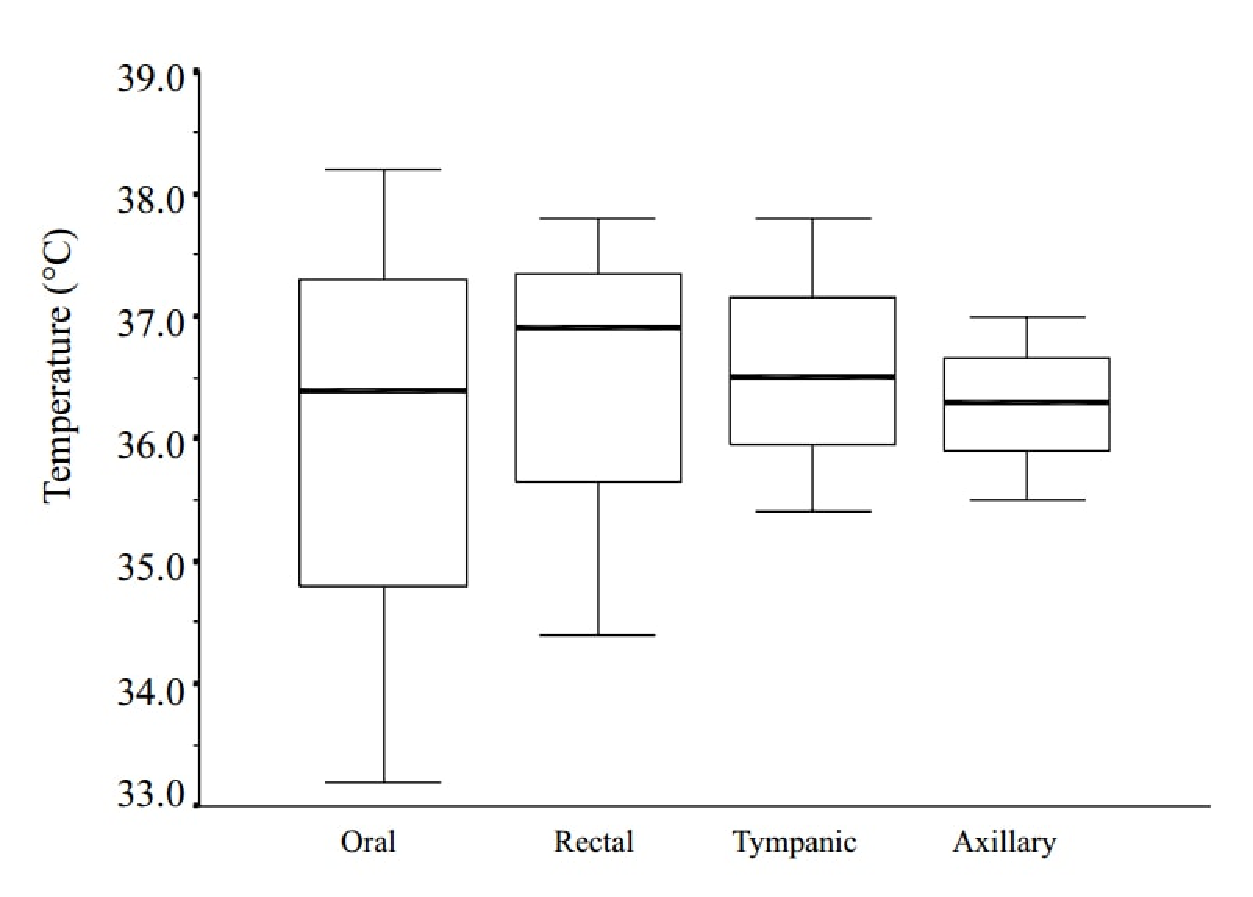
\includegraphics[scale=0.3]{figs/VariationsInTemp}
   \caption{The results from 20 studies with strong or fairly strong evidence of normal oral, rectal and tympanic temperature ($^{\circ}$C) in adult men and women are presented. Temperature is obtainable as mean value(bold lines), 1st and 3rd quartiles (unfilled bars) and range (thin lines).}
   \label{fig:VariationsInTemp}
\end{figure}

Studies have also been done comparing measurements at distinct locations to pulmonary artery temperature in ill patients. A study has shown ear-based  $0.07\pm 0.41$  $^{\circ}C$; urinary bladder  $0.03\pm 0.23^{\circ}C$; oral  $0.05\pm 0.26^{\circ}C$; and axillary $-0.68\pm 0.57 ^{\circ}C$. The accuracy of each method varied with the level of pulmonary artery temperature. Repeated measurements with all four methods had mean standard deviation values within $\pm 0.2^{\circ}C$ \citep{erickson1993comparison}.

A second study done by \cite{lefrant2003temperature} showed the following results: oesophageal  $0.11 \pm 0.30^{\circ}C$, rectal $-0.07 \pm 0.40^{\circ}C$, axillary $0.27\pm 0.45^{\circ}C$, inguinal $0.17 \pm 0.48^{\circ}C$, urinary bladder $-0.21 \pm 0.20^{\circ}C$.

The location of the device in development is restricted to the ear, therefore the tympanic membrane is the preferred location to take temperature measurements. The referenced studies show that the tympanic membrane is a valid location to measure accurate core temperature.


\subsection{Tympanum}

\subsection{Tympanum}

\subsection{Tympanum}

\subsection{Tympanum}










\subsection{Core Temperature}
Thermoregulation is the body's way of keeping its internal temperature within certain bounds to create a favourable environment for chemical reactions to take place. Temperature is controlled by the hypothalamus. Core body temperature is an indication of overall health. Elevated temperature due to a fever can indicate the presents of an infectious disease. It is often the key indication to start treatment or not. Therefore, core temperature measurement is part of a full clinical examination and part of the vital sings group.

The location where temperature is measured is an important factor, for temperature is not constant throughout the body. This is because heat production and heat loss are not constant throughout the body. Extremities are usually cooler than the core. Traditional locations for measuring temperature are the tympanic membrane, axilla, mouth, rectum, oesophagus, forehead and urinary bladder. The mean temperature of these areas varies as well. A systematic literature review done by \cite{sund2002normal} combined the results of 20 studies to identify oral, rectal, tympanic and axillary temperature ranges in healthy humans. Table~\ref{fig:VariationsInTemp} shows the results.



Studies have also been done comparing measurements at different locations to pulmonary artery temperature in ill patients. A study have shown ear-based 0.07 $\pm 1$ 0.41 $^{\circ}$C; urinary bladder 0.03 $\pm 1$ 0.23 $^{\circ}$C; oral 0.05 $\pm 1$ 0.26 $^{\circ}$C; and axillary -0.68 $\pm 1$ 0.57 $^{\circ}$C. The accuracy of each method varied with the level of pulmonary artery temperature. Repeated measurements with all four methods had mean SD values within $\pm 1$ 0.2 $^{\circ}$C \citep{erickson1993comparison}.

A second study done by \cite{lefrant2003temperature} showed the following results: esophageal 0.11 $\pm 1$ 0.30 $^{\circ}$C, rectal -0.07 $\pm 1$ 0.40 $^{\circ}$C,axillary 0.27 $\pm 1$ 0.45 $^{\circ}$C, inguinal 0.17 $\pm 1$ 0.48 $^{\circ}$C, urinary bladder -0.21 $\pm 1$ 0.20 $^{\circ}$C.

According to Harrison's Principles of Internal Medicine (18th ed., normal internal body temperature is 37.0 $^{\circ}$C.



\subsubsection{Temperature Measurement Theory}
Various methods are available for measuring core temperature. Non-electric, fluid-filled thermometers was the first to be used. The mercury-filled thermometer was used by early physicians to study the thermoregulation of the human body and crudely identify fevers. Since then, the mercury has been replaced by coloured alcohol or another heat sensitive liquid, due to toxicity of mercury.

Another type of fluid-filled thermometer is the liquid-crystal thermometer. It contains liquid crystals that changes colour when at different temperatures. The use of these two types of fluid-filled thermometers has decreased significantly due to the accuracy, speed and connivance of digital thermometers.

Electrical thermometers are now the industry standard of measuring core temperature. Medical thermometers are usually classified by the location that they use to make there measurement. For the sake of this study it is also important to obtain an understanding of how they make their measurements. Central to any  thermometer lies a electrical temperature transducer/sensor. Various temperature sensors are available, but the following three are the most commonly used.

Two methods are generally available to capture the temperature of the tympanic membrane. Firstly a contact thermistor and secondly an infra-red sensor. Placing a thermistor in contact with the membrane can cause discomfort and injury to the patient. The infra-red sensor is therefore a better option for is can measure the temperature without making contact with the tympanic membrane.

\subsubsection{Thermocouples}
Thermocouples make use of the thermo-electric effect to make a temperature measurement. They consist of two dissimilar conductors connected at the one end, knows as the measuring junction. The other ends of the two wire are known as the reference junction and are connected to a voltage meter via common conductors. A voltage is generated dependant to the temperature difference between the measuring- and reference junctions.

Thermocouples do not respond to absolute temperature, therefore their accuracy depends on how well the reference temperature can be defined.

Thermocouples can be connected in series and are then called thermopiles. This amplifies the output voltages, resulting 'n a average temperature reading across many sensors (temperature averaging).

Thermopiles can be used to detect thermal radiation. All matter with temperatures above 0K radiates electromagnetic radiation. The wavelength distribution varies according to the temperature of the matter and is described by Planck's law. The temperatures relevant to this study is the core temperature of humans, which is around 37 $^{\circ}$C. According to Planck's law, the theoretical peak density wavelength will be at 12 um (verify ad include formule). This is in the infra red range, and therefore this type of thermal radiation thermometer is called a Infra-Red thermometer.

Emissivity is the ability of an object to radiate thermal energy. Emissivity is a material-dependent property. It is quantified as a ratio of thermal energy emitted by a surface relative to the thermal energy emitted by an ideal black body at the same temperature. A black body is an idealized surface that reflects no radiation, meaning all energy radiated from the surface are due to the temperature of the surface. Thus, a black body have an emissivity of 1 and have the maximum theoretical radiation at a given temperature. The accuracy of an IR sensor depends on the ability of the target object to emit sufficient thermal radiation for the sensor to detect. Therefore, the emissivity of the target object should be close to one.

According to \textbf{source} the emissivity of skin is 0.98.

An IR thermometer generally consists out of a thermophile attached to a blackbody and shielded by an IR filter that also acts as a lens to focus IR waves [16]. This setup, shows in Figure\ref{fig:IR_Thermometer}, allows for the non-contact temperature sensing of the tympanic membrane. Unlike pulse rate, breathing and electrical brain activity, the core body temperature varies slowly. It takes minutes to vary significantly. Therefore, the sampling rate of body temperature can be as slow as 0.5 Hz.

 \begin{figure}
   \centering
   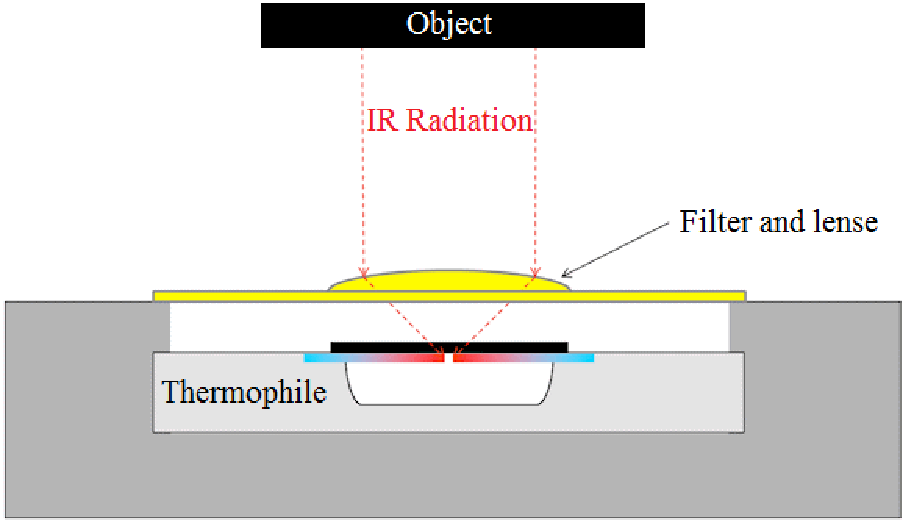
\includegraphics[scale=0.3]{figs/IR_Thermometer}
   \caption{IR Thermometer diagram (V Polyzoev et al: Demystifying Thermopile IR Temp Sensors)}
   \label{fig:IR_Thermometer}
\end{figure}


Thermocouples are widely used in medical thermometers due to their 

\subsubsection{Thermistors}
Thermistors

\subsubsection{Resistance temperature detectors}
Resistance temperature detectors (RTD) 






Another important aspect is the way in with the ele temperature measurement in set op 

Other methods used by the literature

Devices used by literature




enter the test of the TMP006 subsystem word doc that is applicable here...

\subsection{Heart Rate}
The presence of a heart beat is a paramount to the sustain the vital cardiac output supplying blood to the whole body. Heart  rate can be controlled or maintained through two different regulatory systems: The intrinsic conduction system and the nervous system. The intrinsic conduction system works through the rhythmic contraction and relaxation of the heart muscle tissue. The heart rhythm is regulated by the sinoatrial node. The nervous system can influence the heart rate through sympathetic and parasympathetic nerves running from the cardiovascular centres in the medulla oblongata to the heart. The heart beat rate is varied to control the blood flow and blood pressure in the body.

Heart rate is influenced by numerous physiological factors including $O_2$, $CO_2$, $H^+$ levels, blood pressure, stress and exercise. Pathological factors can include fever, sepsis, heart disease and anaemia. Tachycardia is abnormally high resting heart rate, generally above 100 bpm, whereas bradycardia is an lower then normal resting heart rate, usually below 60 bpm. Although these two conditions are not necessarily danger signs, it may be an indication of health problems and therefore heart rate measurement is part of any medical examination and one of the vital signs in humans.

Heart rate can be measured in a variety of ways. Electronic ways of measuring heart rate include electrocardiography (ECG), photoplethysmography (PPG), ballistocardiography(BCG), electronic stethoscopes and Doppler flow-meters.

\subsubsection{Electrocardiography}
ECG records the electrical activity of the heart over a period of time. It is the the recommended way of monitoring heart rate in most intensive care units. A cardiologist will use a 12 lead ECG with 10 electrodes placed in a specific configuration on the chest. Various wearible devices use ECG to measure heart rate. Fitness monitors normally uses a chest strap with electrodes to detect the heart's electrical activity. Studies have been done developing wearable ECGs for clinical use.

The typical telemedicine set-up of a wearable ECG is a signal acquisition module, collecting and sending data by means of a wireless transceiver to a smart-phone, which then uploads the data to a healthcare server \citep{wang2010wearable} and/or \citep{prawiro2016integrated}. %Maybe put this paragraph in a design related chapter

The latest in wearable ECK systems is the use of Dry Polymer-based electrodes \citep{wang2010wearable} or non-contact electrodes that can be place on top of clouthing \citep{lin2013development}. This is an improvement above the standard conductive gels or adhesives and can be used repeatedly. But these electrods still needs to be place on the chest. An ear located ECG monitor have been developed by \cite{winokur2012wearable}. This device uses an one lead set-up with on electrode place on the mastoid bone and one on the neck. This configuration relies on the conductive properties of human tissue to carry electrical charges form the heart to the location of the ear. (See also: Bluetooth Low Energy (BLE) Based Mobile Electrocardiogram Monitoring System; 

\subsubsection{Photoplethysmography}
Photoplethysmography (PPG) is an optically obtained  plethysmogram (volume change of an organ). PPG can be used to measure the change in volume of blood vessels close to the skin surface. When the left ventricle contracts a pressure pulse propagates through the arteries from the heart to the extremities of the body. This wave corresponds to the systolic blood pressure. Blood vessels walls contain elastic fibres that allow them to stretch. This means that the diameter of vessels will increase when the blood pressure increase, causing   arteries so to stretch and contract with each heartbeat. A PPG can be used to measure this variation.

According to Lambert's law, the amount of light absorbed is proportional to the length of the path that the light has to travel in the absorbing substance. Therefore a change in blood vessel diameter will cause a change in tissue absorption. Light shined through the skin to illuminate the underlying subcutaneous tissue can either be reflected, absorbed or allowed to transmit through the tissue. Changes in the light absorption of the tissue can be detected by measuring this reflected or transmitted light. As defined by Lambert's law: changes in absorbed light is due to the changes in arterial diameter and thus, an indication of the pulse. Figure of reflective and transmittance PPG.

A photoplethysmogram of blood vessels is obtained through pulse oximetry. A pulse oximeter consiste of a light emitter and detector. It can operate in reflectance or transmittance modes as shown in Figure~\ref{fig:PulseOxiModes}. Transmittance pulse oximetry measures the light that is allowed to transmit through the tissue. It is more common, but its placement is restricted to a thin part of the patient's body that will allow light through. Reflectance pulse oximetry has no such restrictions for it measures the light that is reflected by the tissue.

\begin{figure}
   \centering
   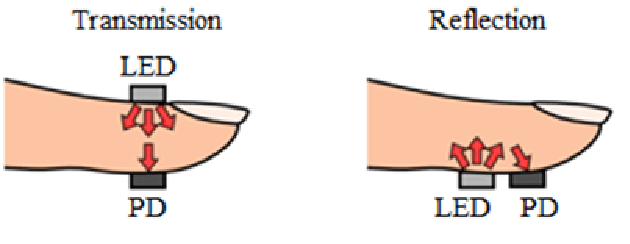
\includegraphics[scale=1]{figs/PulseOxiModes}
   \caption{Pulse oximetry in reflective or transmittance modes}
   \label{fig:PulseOxiModes}
\end{figure}

The signal read by the photo detector of the pulse oximeter consists of a AC component superimposed on a DC signal. The DC component is the constant reflection of light by the body's tissue: skin, fat, venous blood and the non-pulsating arterial blood. The AC components is the variation in reflected light due to the change in diameter of the arteries and is usually between 0.5 - 2\% of the DC component  \citep{tavakoli2006analog}. Therefore the frequency of the AC component is synchronised to the heart rate.

\subsubsection{Ballistocardiography}
Ballistocardiography (BCG), also known as a seismocardiogram, is the measurement of the mechanical effects of the beating heart. Typically accelerometers or pressure sensors will be used to measure movement or forces on the surface of the body. BCG has been researched for use in ear heart rate extraction. In a wearable device proposed by \cite{da2010ear}, mechanical vibrations associated with heart rate are converted to electronic signals through capacitive sensing electrodes. This method works my measuring the change in capacitance between the two electrods as the distance between them changes due to heart rate vibrations. A study by \cite{winokur2012wearable} proposed measuring the head-to-foot axis recoil during the principal blood-volume shift during cardiac ejection. This is done by placing an MEMS accelerometer behind the auricle. Due to the movement dependent method of operation this technology is extremely susceptible to motion artefacts and it can only be used during which the body is stationary.


The traditional and simplest of which is placing an index and middle finger on the wrist and counting the arterial pulses felt per minute. In fact, heart rate pulse can be felt throughout the body where large arteries are close to the skin.

A variation of this technology is discussed in a article by \cite{park2015wearable}. They propose using a scissor shaped hinge mechanism in the ear canal that measures the change in the canal size due to the in-ear blood pulse waves. The mechanical movement it converted to an electrical signal through a piezoelectric film sensor.

\subsubsection{Other methods}
Electronic stethoscopes uses an microphone to record heart sounds. The hears makes a distinct series of sounds during the cardiac cycle due to blood turbulence and the shutting of heart valves. The period of this sound series can be used to determine heart rate and does not require skin-contact.

A Doppler flow-meter can be used to detect the alternating blood current component in near-surface arteries. This component is synchronised to the heart rate frequency. The device can use ultrasound, microwaves of light to achieve the Doppler shift.

\subsection{Respiratory rate}
Breathing is a process critical for life. Respiration is the first step in the chain of events to get oxygen to the body's cells for metabolism to provide the body with energy. Breathing and plus it the first signs of life to check for in a medical emergency. %Say this better

How is the RR controlled

Appart form the obvious face that a lack of breathing is a problem, the RR can divulge some information about a persons health. What does the RR tell us about health


Measure through baseline oscillations of BCG signal (see The Ear as a Location for Wearable Vital Signs Monitoring \citep{da2010ear})

Respiratory rate is the rate at which ventilation takes place in the lunge. One inhalation and exhalation cycle is counted a breath and respiratory rate is usually measured in breaths per minute. Healthy adults have an resting respiratory rate of between 12 and 18 breaths per minute., This can vary drastically if a the body is experiencing physical or emotional stress.

It is important to monitor breathing, for irregular breathing or difficulty to breathing may be an induction of healthy problems. Apnoea is when breathing stops completely. This is especially an danger in infants and patients in the ICU.

Traditionally, respiratory rate is measured by counting the number of timer the chest visibly rises as a person inhales. Other methods include listening to the chest with a stethoscope and counting audible breaths, fixing an accelerometer to the chest, measuring CO\textsubscript{2} levels in the respiratory gases and looking at variations in heart rate.

Caretakers are usually very concerned about sleep apnoea in infants, as cause a risk for infant mortality. Apnoea monitors are available to warn caretakers if breathing halts. These monitors usually measure force or acceleration caused by the breathing of the sleeping infant. The device can be worn by the infant or can by placed in the cot.


All respiratory related measurements in the reviewed products rely on movement sensors attached to the body of the infant that senses its movement. Sensors include accelerometers and the \textit{BreathOptic}\textsuperscript{\texttrademark} sensor used by Sleep-Mat. These sensors detect the chest movement produced by the infant while breathing. In some cases, like Mimo and Sleep-Mat, these sensors are sensitive enough to determine the infant's respiratory rate from this movement. In other products, such as Anglecare and Monbaby, the sensors are sensitive enough to register the movement due to breathing, but not sensitive enough the extract the rate of breathing.
Alerts are sent wirelessly to the cellphone of the caretaker if the movement stops for a certain amount of time. This may indicate that the infant has stopped breathing. The problem with this method is that products like Monbaby, Anglecare and Mimo will only alert the caretakers once the infant has stopped breathing completely for 15 or 20 seconds. This may be too late to prevent an infant mortality. A product is needed that can accurately monitor the respiratory rate and warn the doctor or caretakers if the respiratory rate drops or becomes irregular.
Respiratory sinus arrhythmia (RSA) is the baseline oscillation in heart rate in synchrony with the respiratory rate. It is observed as an increase in heartrate during inspiration and a decrease during expiration. According to a study done by Stratton JR et al, the variation in heart rate due to RSA is higher in younger test subjects with 74\% increase in children vs. 52\% increase in adults [5]. These findings support the use of RSA to determine the infant's respiratory rate. A study has been done by D da He investigating the use of ballistocardiogram heart rate measurements to detect RSA [6]. This project will attempt to detect RSA in pulse oximetry heart rate measurements. This is a unique approach in wearable monitoring devices. The advantage is that no extra sensors, like accelerometers, are needed for the measurement of respiratory rate.

\subsection{Blood Oxygen Saturation}
Haemoglobin is the oxygen transporter protein found in the red blood cells of blood. Blood gets oxygenated in the lungs and then carries \(O_2\) to the rest of the body for aerobic respiration necessary to produce energy. The correct levels of oxygen in the blood is vital to the health of the individual.

Oxygen saturation ($SO_2$) refers to the fraction of oxygenated haemoglobin to total haemoglobin in the blood: $$ SO_2 = \frac{C(HbO_2)}{C(HbO_2)+C(Hb)}\times100\% $$ Where $ C(HbO_2) $ is the concentration of deoxygenated haemoglobin (deoxyhaemoglobin) and $ C(Hb)$ is the concentration of oxygenated haemoglobin (oxyhaemoglobin).

Blood oxygen saturation of 95-100\% is normal in healthy humans. Hypoxemia is the condition when the saturation is below 90\%. This can be an indication of circulatory or ventilatory problems, anaemia or sleep apnoea. Levels below 80\% can hinder organ function and can lead to organ failure, cardiac- or respiratory arrest. In the absence of oxygen, damage to the brain starts within 5 minutes with brain death ensuing within another 10 to 15 minutes.

Oxygen saturation can be measured by means of an arterial blood gas test resulting an arterial oxygen saturation reading. An alternative method is pulse oximetry. This method measures peripheral capillary oxygen saturation (Sp02). This is a clinically excepted estimation of the arterial oxygen saturation.

Various devices are available for measuring blood oxygen saturation. Elaborate...

\subsubsection{Oxygen Saturation Measurement Theory}
Blood oxygen saturation calculation through pulse oximetry relies on the different adsorption spectra of oxyhaemoglobi) and deoxyhaemoglobin. Figure~\ref{fig:AbsorptionSpectra} shows the absorption spectra of oxy- and deoxyhaemoglobin. It can be noted that deoxyhaemoglobin has a significantly higher absorption of red light (600 - 750 nm wavelength) while oxyhaemoglobin has a slightly higher absorption of infrared light (850 - 1000 nm wavelength). This explains the fact that oxyginated blood apperas bright red and deoxygineted blood is a darker shade of red. (find a source for the image) (What is on y-axis and what is NIR region). Literature usually uses 660 nm (red) and 940 nm (near infrared) http://www.iosrjournals.org/iosr-jeee/Papers/Vol8-issue1/D0812226.pdf?id=7592

\begin{figure}
   \centering
   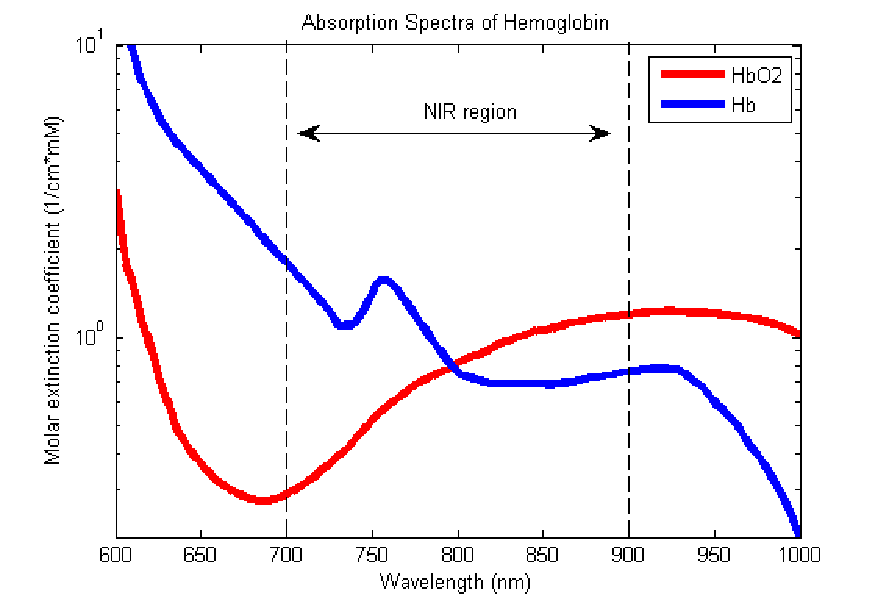
\includegraphics[scale=0.8]{figs/AbsorptionSpectra}
   \caption{Absorption spectra of oxy- and deoxyhemoglobin}
   \label{fig:AbsorptionSpectra}
\end{figure}

From the Figure~\ref{fig:AbsorptionSpectra} it can be seen that the ratio of absorbed red light to absorbed infra-red light is unique to a certain level of blood oxygen saturation. Therefore this ration can be used to estimate blood oxygen saturation. To account for different DC absorption between patients, a modulated ratio ($R$) is used:
$$R = \frac{\left(\frac{AC}{DC}\right)\textsubscript{red}}{\left(\frac{AC}{DC}\right)\textsubscript{IR}} $$
This ensures that the $ O_2 $ saturation of only the arterial blood is calculated. The ration can be checked against an empirical determined curve. The standard formula for this curve is found in literature as $ \% SpO_2 = 110-25R $, (http://www.ti.com/lit/an/slaa655/slaa655.pdf) but it can vary from device to device. 

\subsection{Respiratory Rate}


\subsection{Respiratory Rate Theory}

\subsection{EEG}

\subsection{EEG Theory}

\chapter{Theory Literature Review}
\label{chp:TheoryLit}
This chapter will accumulate a thorough understanding of the theory and current state of technology relevant to the measurement of each medical sign required of the Ear-Monitor. Attention will be given to the different methods available to determine each medical sign. This section will also make reference to various articles and studies done by other researchers in this field of study. The aim is to gather all the relevant information in order to make an informed selection of the methods and sensors the Ear-Monitor will use to measure each medical sign.

\section{Core Temperature}
Various methods are available for measuring core temperature. Non-electric, fluid-filled thermometers was the first to be used. The mercury-filled thermometer was used by early physicians to study the thermoregulation of the human body and crudely identify fevers. Since then, the mercury has been replaced by coloured alcohol or another heat sensitive liquid, due to toxicity of mercury.

\medskip

Another type of fluid-filled thermometer is the liquid-crystal thermometer. It contains liquid crystals that changes colour when at different temperatures. The use of these two types of fluid-filled thermometers has decreased significantly due to the accuracy, speed and connivance of digital thermometers.

\medskip

Electrical thermometers are now the industry standard of measuring core temperature. Central to any digital thermometer lies a transducer that convert temperature to an electrical signal. Resistance temperature detectors, thermocouples thermistor and thermopiles will be discussed. They can be divided into contact and non-contact thermometers.

\subsection{Contact Thermometers}
These are a family of thermometers that measure their own temperature with the assumption they and the object whose temperature is of interest, are in thermal equilibrium. Therefore, they are usually placed in contact with the object. When using a contact thermometer in the ear, the sensor part of the thermometer can be placed in contact with the ear canal wall, the air inside the canal or with the tympanic membrane self.

\subsubsection{Resistance Temperature Detector}

Resistance temperature detectors (RTDs) uses the temperature-resistance relationship for metals to measure temperature. Thin wire coils or films of platinum, copper or nickel are usually preferred for they have a stable and repeatable temperature-resistance relationship over a large temperature range.

\subsubsection{Thermocouple}
Thermocouples make use of the thermo-electric effect to make a temperature measurement. They consist of two dissimilar conductors connected at the one end, knows as the hot junction (measuring junction). The other ends of the two wires are known as the cold junction (reference junction) and are connected to a voltage meter via common conductors. A voltage is generated dependant to the temperature difference between the measuring- and reference junctions. Thermocouples do not respond to absolute temperature; therefore, their accuracy depends on how well the reference temperature can be defined. Reference temperatures are usually determined by a precise thermistor. Thermocouples are very versatile and widely used in clinical applications, but the downsides are that their output signal is low and non-linear, therefore requiring a sensitive and stable voltage measuring device \citep{jones2010biomedical}.

\medskip

Thermocouples can be connected in series and are then called thermopiles. This configuration sums the output voltages, resulting in temperature averaging. This method improves accuracy by reducing noise. 

\subsubsection{Thermistor}
A thermistor is a type of semiconductor whose resistance varies with changes in temperature. They differ from RTDs in that they are usually made of ceramics, they have higher precision over a smaller temperature range and they can have a negative relation to temperature. Thermistors are preferred above RTDs and thermocouples for use as biomedical sensors due to their faster response time and higher sensitivity over a smaller range and. The smaller range does not matter, for the temperature range of interest in biosensors are small and well defined. 

\subsubsection{Contact Thermometer Application}
In the case of RTDs and thermistors, the measuring element is placed in position and a current is sent through the sensor. By measuring the voltage across the resistive element, it is possibly to calculate the voltage and subsequently determine the temperature. In the case of the thermocouple, the hot junction can be placed in contact with the canal wall or tympanum. Typically, the hot junction will be enclosed with a soft material to protect the canal and tympanum. The canal is sealed off and time is allowed for the area to equilibrate to tympanic temperature.

\medskip

Placing a thermometer in contact with the tympanic membrane will give an accurate measurement, but can cause discomfort to the wearer. There is also a risk of harming the tympanic membrane. Sensors in contact with the ear canal wall or the air inside the canal run the risk of making errors by measuring the temperature of objects that are not in thermal equilibrium with the tympanic membrane. Therefore, non-contact thermometers will be considered.

\subsection{Non-contact Thermometers}
Thermopiles can be used to detect thermal radiation without being I contact with the object. All matter with temperatures above 0 K radiates electromagnetic radiation according to the Stefan-Boltzman law. The thermal radiation, $Q$, per unit area is given by the equation:

$$Q=\varepsilon \sigma T^4.$$

Where $\varepsilon$ is the emissivity, $\sigma$ the Stefan-Boltzman constant and T the temperature of the object.

The wavelength distribution varies according to the temperature of the object and is described by Planck's law:

$$B_\lambda (\lambda ,T)=\frac{2hc^2}{\lambda ^5}\frac{1}{e^\frac{hc}{\lambda k_B T} -1}.$$
 
Where $B_\lambda$ is the spectral radiance, $\lambda$ the radiation wavelength, $h$ Planck's constant, $k_B$ Boltzman's constant $c$ the speed of light and $T$ the object's temperature. Through maximizing $B_\lambda$ , it is possible to find the dominant wavelength that is emitted at a certain temperature. Figure~\ref{fig:PlancksLaw} shows a plot made of spectral radiance versus wavelength at $T=$ 37 $^{\circ}C$, the core temperature of humans. It can be seen that the dominant wavelength is at 9.35 $\mu$m. This is in the infrared range, and therefore this type of thermal radiation thermometer is called an infrared thermometer.

\medskip

 \begin{figure}[h]
   \centering
   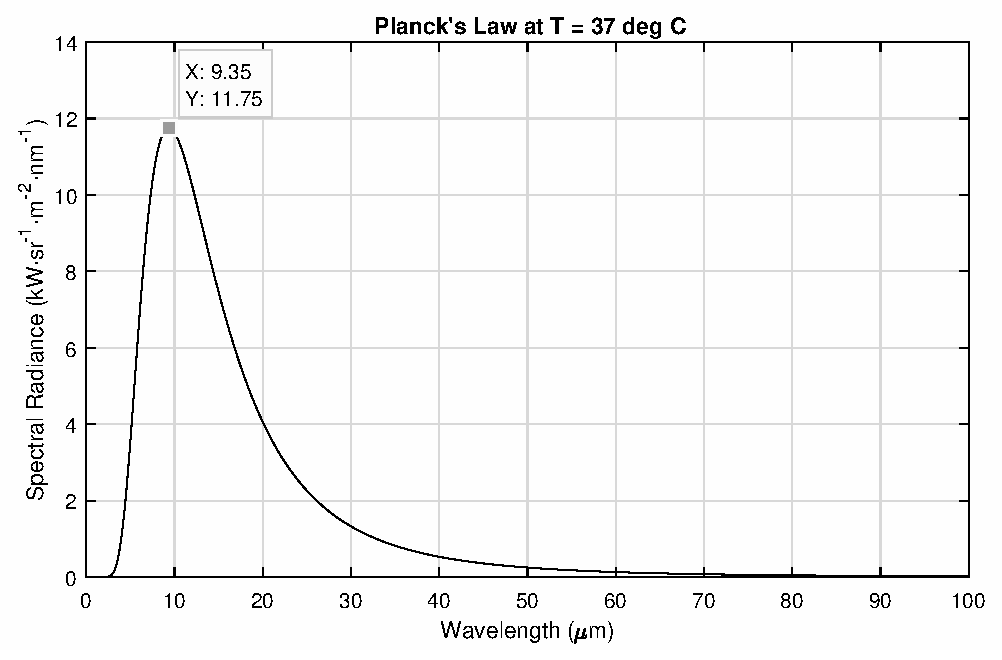
\includegraphics[scale=0.6]{figs/PlancksLaw}
   \caption{Plot showing how Planck's law can be used to determine the dominant radiation wavelength at certain temperature}
   \label{fig:PlancksLaw}
\end{figure}

In the case of measuring the temperature of the tympanic membrane, the hot junction's temperature will be determined by the radiation received from the tympanum minus the radiation radiated by the sensor self.

\medskip

When talking about thermal radiation, an important aspect is emissivity. Emissivity is the ability of an object to radiate thermal energy. It is quantified as a ratio of thermal energy emitted by a surface relative to the thermal energy emitted by an ideal black body at the same temperature. A black body is an idealized surface that reflects no radiation, meaning all energy radiated from the surface are due to the temperature of the surface. Thus, a black body have an emissivity of 1 and have the maximum theoretical radiation at a given temperature. The accuracy of an infrared sensor depends on the ability of the object to emit sufficient thermal radiation for the sensor to detect. Cross-referencing various emissivity tables, it was found that the emissivity of human skin is 0.98, meaning that it is an excellent emitter of thermal energy \citep{stumme2003emissivity} \citep{EmissivityThermoWorks} \citep{EmissivityOptotherm}. The ear drum is covered with skin, making it an ideal target object for a non-contact thermometer.

\medskip

An infrared thermometer generally consists out of a thermophile attached to a blackbody and shielded by an infrared filter that also acts as a lens to focus infrared waves \citep{irTempSensors}. This setup, shows in Figure \ref{fig:IR_Thermometer}, allows for the non-contact temperature sensing of the tympanic membrane. Unlike pulse rate, breathing and electrical brain activity, the core body temperature varies slowly. It takes minutes to vary significantly. Therefore, the sampling period of core temperature can be as long as 10 seconds.

\medskip

\begin{figure}
   \centering
   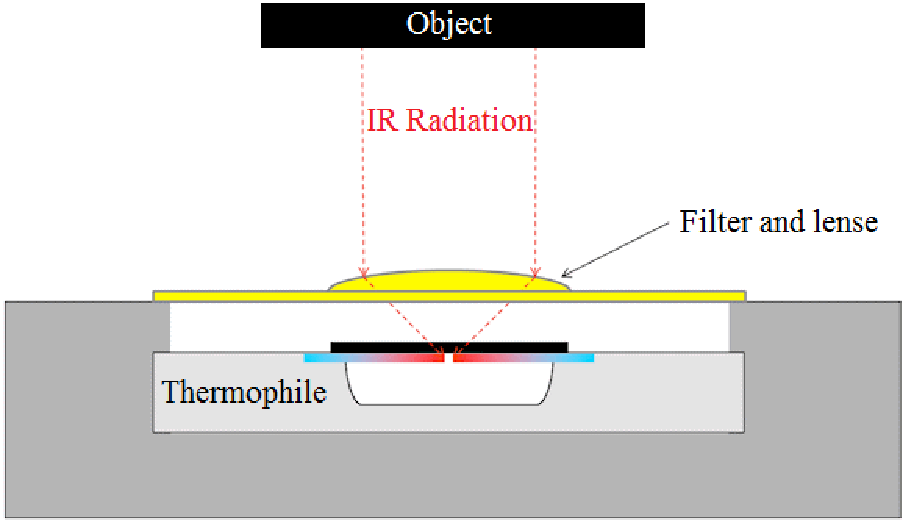
\includegraphics[scale=0.5]{figs/IR_Thermometer}
   \caption{IR Thermometer diagram (V Polyzoev et al: Demystifying Thermopile IR Temp Sensors)}
   \label{fig:IR_Thermometer}
\end{figure}

\subsection{Commercial Temperature Monitoring Devices}
Ear thermometers are widely used at home and in hospitals. Ear contact thermometers like Novatemp\textsuperscript \textregistered{} and Starboard\textsuperscript \textregistered{} claims a $\pm$0.2 $^{\circ}C$ accuracy. Non-contact infrared ear thermometers usually have a similar rated accuracy. None of these are, however, wearable devices. 

\medskip
 
The \textit{degree}$^{\circ}$, Figure \ref{fig:Degree}, is a continuous in-ear thermometer for children, developed by \textit{cosinuss}$^{\circ}$, a company specialising in wearable sensors. The bulk of the device is worn behind the ear, and there is a wire running over the auricle to the ear canal, in which a probe is placed. The device takes its temperature measurements with a sensor placed in contact with the canal wall. The manufacturer claims an accuracy of $\pm$0.1 $^{\circ}C$. It monitors temperature continuously and sends real time data to a mobile phone.

\medskip

\begin{figure}[h]
   \centering
   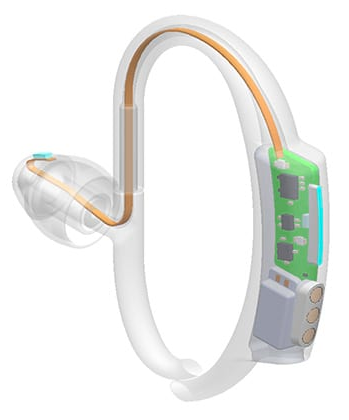
\includegraphics[scale=0.5]{figs/Degree}
   \caption{CAD model of the \textit{degree}$^{\circ}$ from the \textit{cosinuss}$^{\circ}$ website (include ref)}
   \label{fig:Degree}
\end{figure}

Apart from the \textit{degree}$^{\circ}$, there are not much literature on wearable ear thermometers. Two patents were found describing similar devices: US 6556852 B1 and US 20090221888 A1. The first of which proposes the use of an infrared sensor pointed at the tympanic membrane, and the latter not specifying the method of measuring. Hopefully, the tests planned for this study can add to this insufficient body of knowledge.

\section{Heart Rate}
The heart is a very dynamic organ whose influence can be felt throughout the body. Therfore there are many options available to monitor heart rate. Electronic monitoring methods include electrocardiography (ECG), photoplethysmography (PPG), ballistocardiography(BCG), phonocardiography and doppler flow-meters.

\subsection{Electrocardiography}
ECG is a recording of the electrical activity of the heart over a period of time. Electrical activity arise from the depolarization and repolarization of the heart muscle during the cardiac cycle. The most prominent electrical charge is the QRS complex, which corresponds to the ventricular depolarization and is visible on the electrocardiogram as a sharp peak in the millivolt range. ECG is the the recommended way of monitoring heart rate in most intensive care units. A cardiologist will use a 12 lead ECG with 10 electrodes placed in a specific configuration on the chest. Various wearable devices use ECG to measure heart rate. Fitness monitors normally uses a chest strap with electrodes to detect the heart's electrical activity. Studies have been done developing wearable ECG devices for clinical use.

\medskip
The latest in wearable ECG electrodes is the use of dry polymer-based materials \citep{wang2010wearable} or non-contact electrodes that can be place on top of clothing \citep{lin2013development}. This is an improvement above the standard conductive gels or adhesives and can be used repeatedly. But these electrods still needs to be place on the chest.

\medskip
An ear located ECG monitor have been developed by \cite{winokur2012wearable}. This device uses a single lead set-up with one electrode place on the mastoid bone behind the ear and a reference electrode placed on the neck. This configuration relies on the conductive properties of human tissue to carry electrical charges form the heart to the ear. They where able to used the electrocardiogram in conjunction with PPG and BCG to determine various heart intervals and track changes in mean arterial blood pressure. Figure \ref{fig:Winokur} shows \cite{winokur2012wearable}'s device and a plot of its electrocardiogram. No heart rate information was extracted.

\medskip

\begin{figure}[hb]
   \centering
   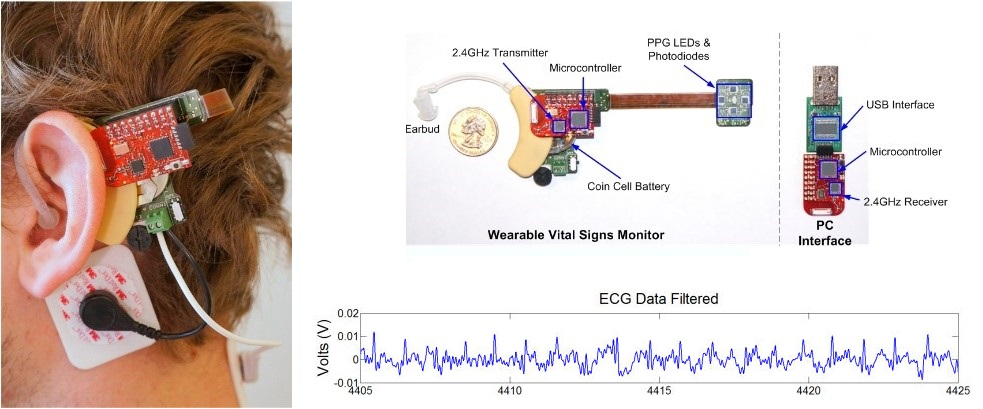
\includegraphics[scale=0.5]{figs/Winokur}
   \caption{Ear-worn device developed by \cite{winokur2012wearable}}
   \label{fig:Winokur}
\end{figure}

\subsection{Photoplethysmography}
PPG produces an optically obtained plethysmogram, which is a plot of volume the change of an organ over time. PPG can be used to measure the change in the volume of blood vessels close to the skin surface. When the left ventricle contracts a pressure pulse propagates through the arteries from the heart to the extremities of the body. This wave corresponds to the systolic blood pressure. Blood vessels walls contain elastic fibres that allow them to stretch. This means that the diameter of vessels will increase when the blood pressure increase, causing arteries to stretch and contract with each cardiac cycle. PPG can be used to determine heart rate by measuring this volumetric variation.

\medskip
A photoplethysmograph can non-invasively determine peripheral arterial blood volume by shining light through the skin surface, into the dermis and subcutaneous tissue and collecting the light transmitter or reflected. Light shined into the tissue can either be reflected, absorbed or allowed to transmit through. This leads to the two modes of PPG operation depicted by Figure \ref{fig:PPGModes}.

\medskip
 
\begin{figure}[h]
\centering
\graphicspath{{figs/}}
%\def\svgwidth{200pt}
\input{figs/PPGModes.pdf_tex}
\caption{The two modes of Photoplethysmography \citep{tamura2014wearable}}
\label{fig:PPGModes}
\end{figure}

In (a) the emitter and detector faces each other and are separated by tissue that can transmit the light, leading to a transmission mode PPG. Transmittance mode PPG is limited to locations on the body where transmitted light can be detected, like the finger, ear lobe, concha and tragus. These locations have limited blood profusion, especially at low temperatures. In (b) the emitter and detector is placed on the same plane and both faces toward the tissue. Light from the emitter is reflected by the tissue and captured by the detector, leading the reflection mode PPG. The emitter and collector needs to be optically isolated so that light cannot pass from the one to the other without going through the tissue. Reflectance mode PPG can be used at more locations, but they are more susceptible to motion artefacts \citep{tamura2014wearable}.

\medskip
According to Lambert's law, the amount of light absorbed is proportional to the length of the path that the light must travel in the absorbing substance \citep{lambertANDbeer}. Therefore, a change in blood vessel diameter will increase the distance the light must travel causing a change in light absorption. This can be detected by measuring reflected or transmitted light. Variation in the light reflected or transmitted will be synchronised with the heart rate.

\medskip
Shorter light wavelengths are mostly absorbed by the tissue, while longer wavelengths can penetrate deeper. Red and near infrared light are preferred for transmission PPG. While green light is becoming more popular for shallow reflectance PPG, due to larger light variations during the cardiac cycle and less noise than near infrared PPG \citep{tamura2014wearable}.

\medskip

The signal read by the photo detector of the pulse oximeter consists of a AC component superimposed on a DC signal. The DC component is the due to the constant transmission or reflection of light by the body's tissue: skin, fat, venous blood and the non-pulsating arterial blood. The AC components is the variation in transmitted or reflected light due to the change in diameter of the arteries and therefore, synchronised to the heart rate. The AC component is usually between 0.5 - 2\% of the DC component \citep{tavakoli2006analog}. Figure \ref{fig:PPG} illustrates the way in which which the heart rate is visible in a photoplethysmograph. It can be seen that the blood volume increase with each heartbeat, and that this causes more light to be absorbed, thus less detected by the photodiode.

\medskip

\begin{figure}[h]
   \centering
   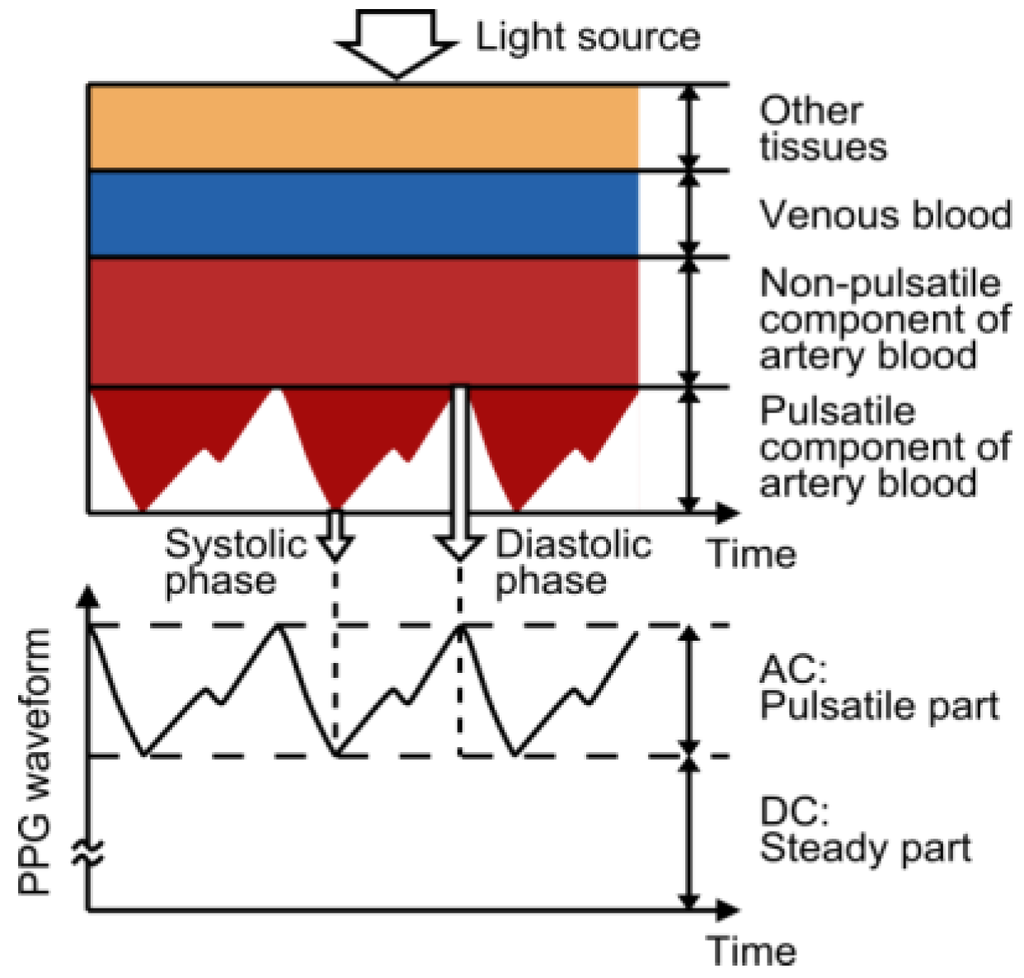
\includegraphics[scale=1.6]{figs/PPG}
   \caption{Pulse oximetry diagram (Source: tamura2014wearable)}
   \label{fig:PPG}
\end{figure}

\subsubsection{Work done by others in Ear PPG}
At this point, PPG is the most attractive option for the Ear-Monitor to measure heart rate and it is given extra attention during the literature review.  A review of work done by others in the field of ear PPG revealed six devices relevant to this study.

\medskip
\cite{shin2009novel} presents a wearable music headset with an integrated transmission PPG ear clip that attaches to the ear lobe. The device includes an accelerometer to aid in the removal of motion artefacts. Evaluation was done through a study comparing the HR from the devise to that made with a conventional ECG recorder. This study revealed a heart rate error of 0.6\% was found.

\medskip
\cite{poh2010motion} designed a wearable PPG with a magnetic earring sensor. The bulk of device sits in front ear canal and held in place by the auricle. A reflective PPG sensor is held against the ear lobe by placing a magnet on the opposite side. The device also includes an accelerometer to make baseline measurements for motion artefact cancellation. A study was conducted to compare the PPG signals measured by the wearable device to chest ECG signals collected by a FDA-approved commercial system. Whilst standing motionless, the study found a very high agreement between the ear PPG and the chest ECG with a mean bias of 0.62 $\pm$ 4.51\% with ECG reference measurements.

\medskip

\begin{figure}[h]
   \centering
   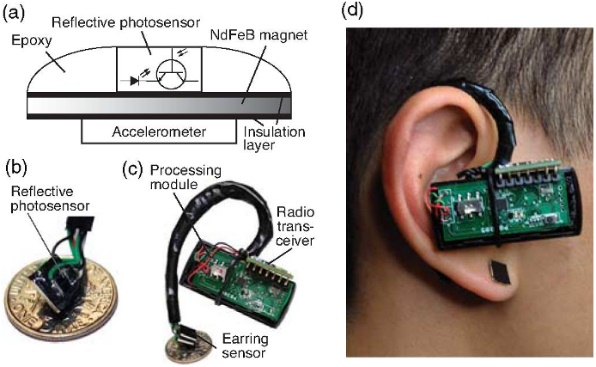
\includegraphics[scale=1.2]{figs/poh}
   \caption{Pulse oximetry diagram (Source: tamura2014wearable)}
   \label{fig:poh}
\end{figure}

\cite{da2010ear} researched an ear worn heart rate monitor containing PPG sensor in reflectance mode. Red light is shined into the tissue behind the ear and collected by a photodiode chip with an integrated transimpedance amplifier. Signals were not digitalised on the device, but recorded and processed on MATLAB. They compared their collected signal with a transition finger PPG and a chest ECG. Figure \ref{fig:DaHe} shows this comparison.

\medskip

\begin{figure}[h]
   \centering
   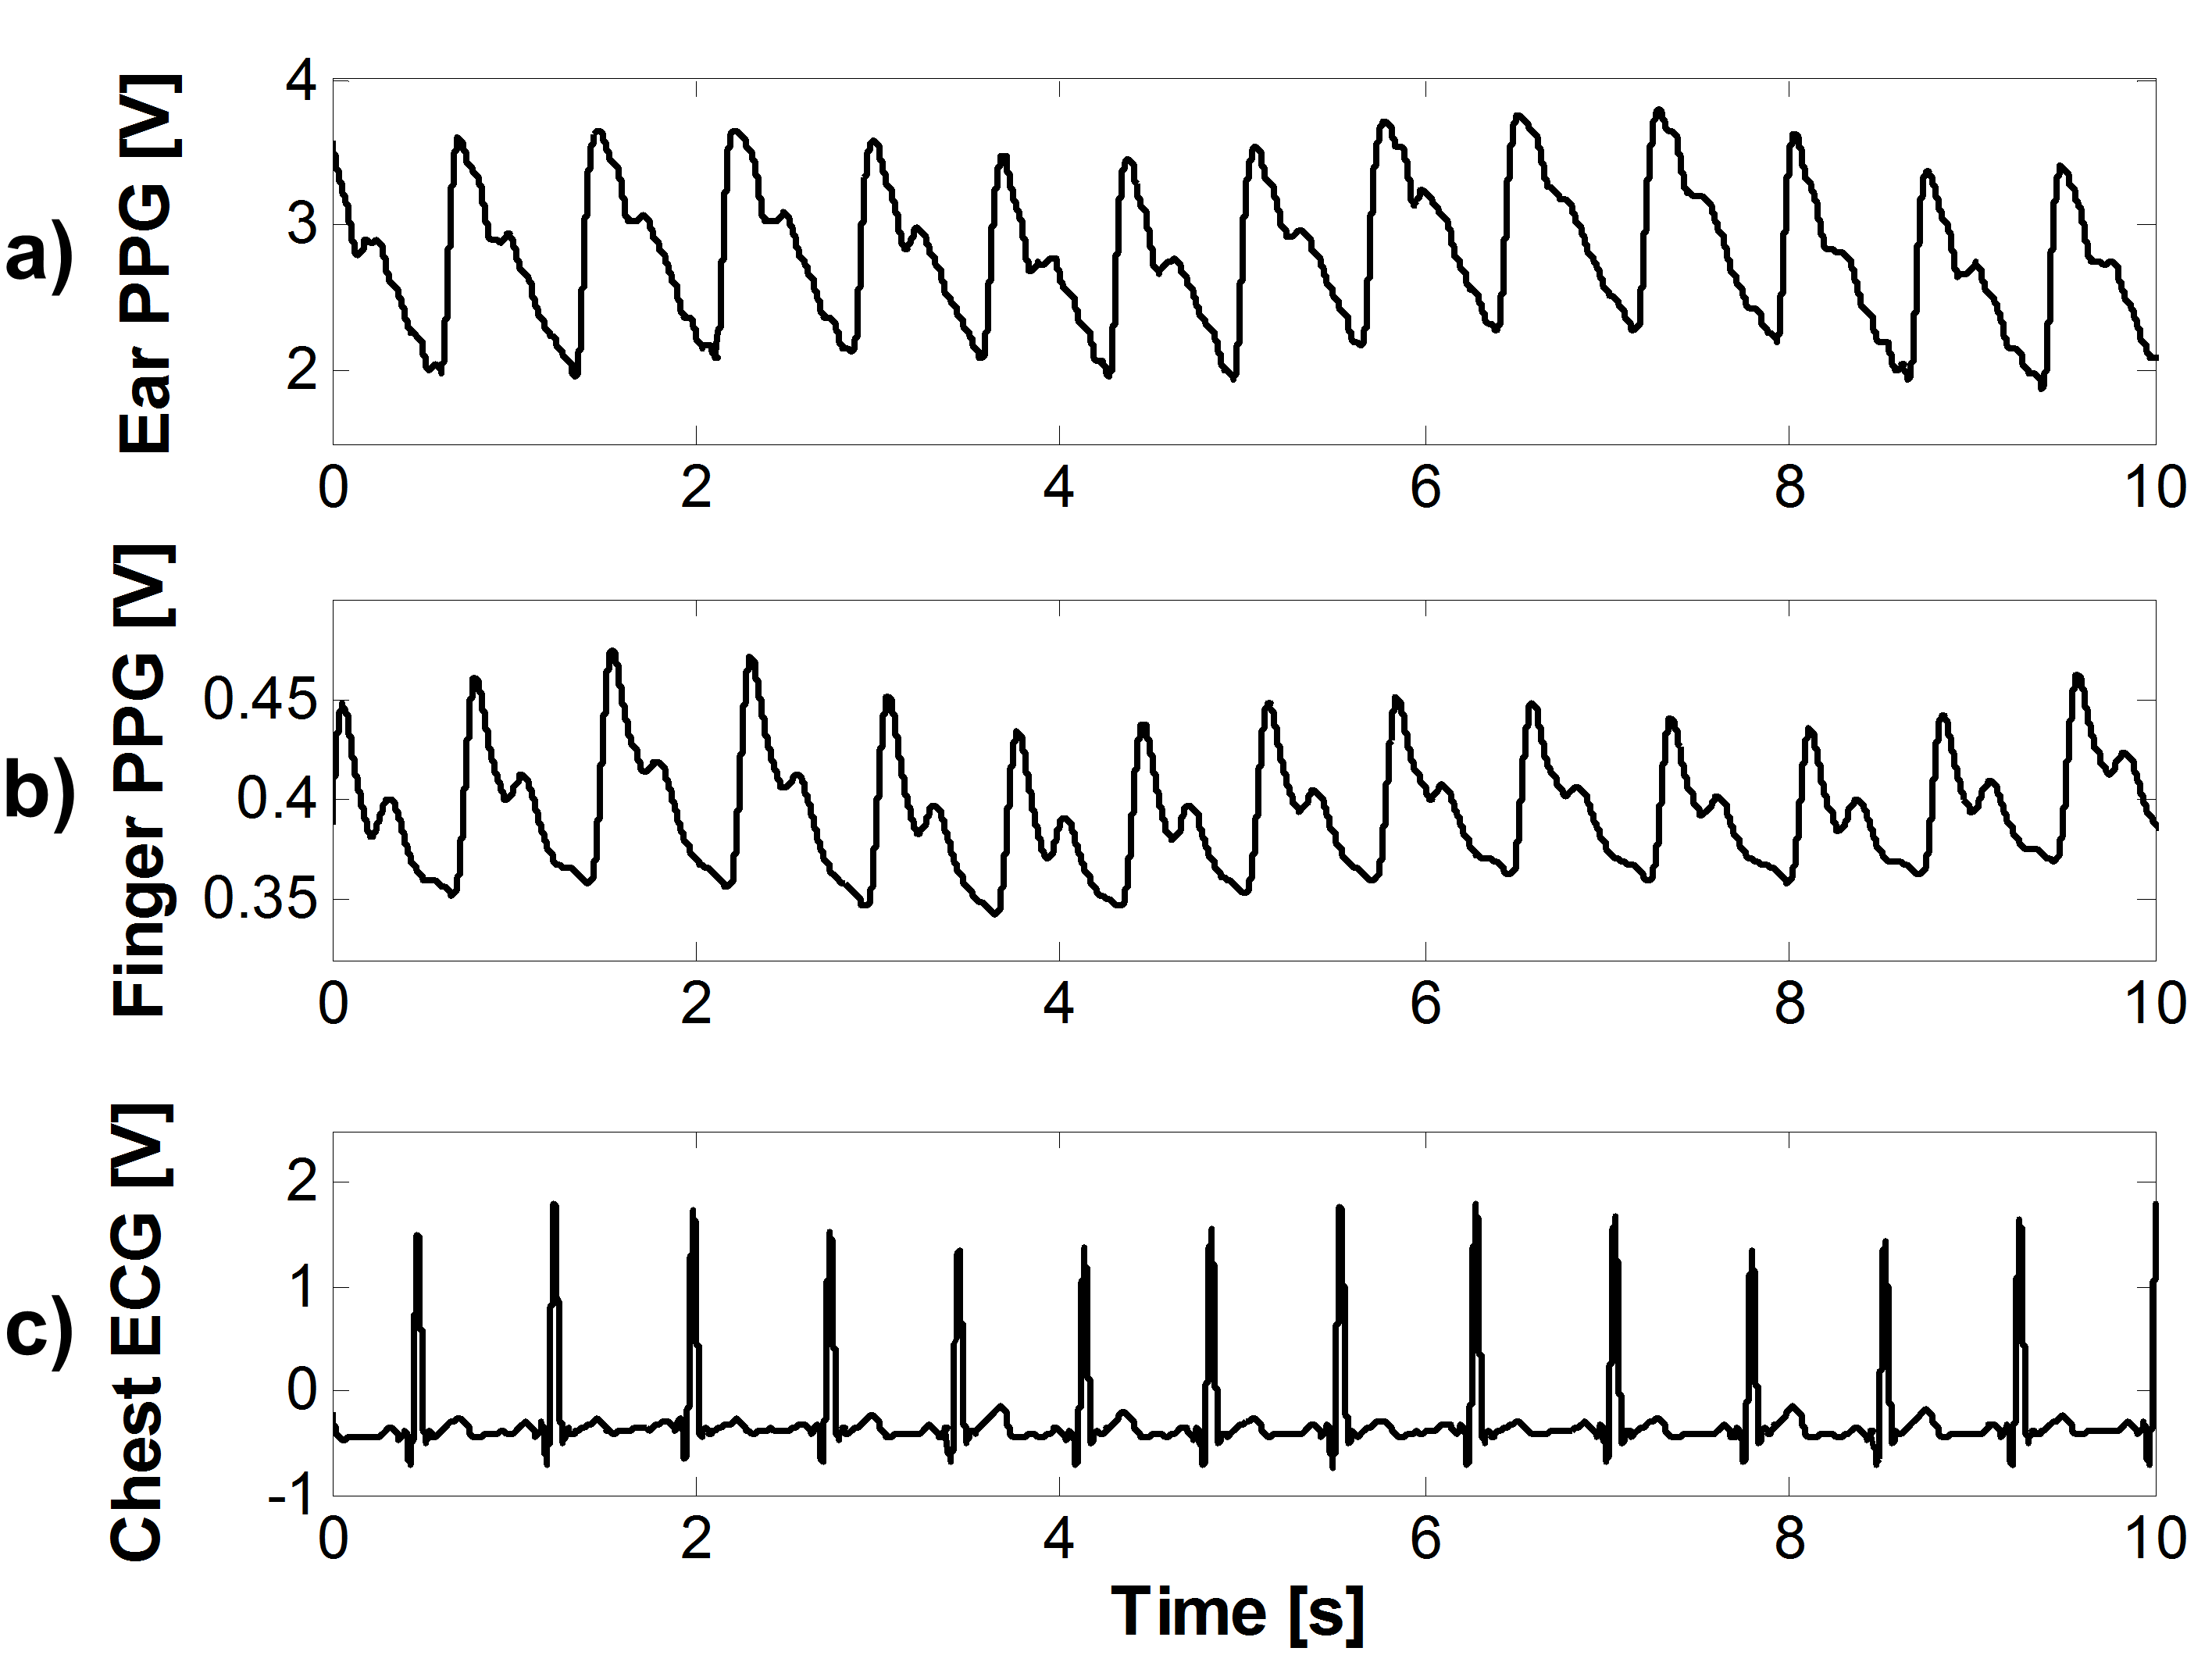
\includegraphics[scale=0.15]{figs/DaHe}
   \caption{Pulse oximetry diagram (Source: tamura2014wearable)}
   \label{fig:DaHe}
\end{figure}

\cite{winokur2012wearable} developed a similar device that shines 660nm and 940nm light waves through tissue at the mastoid bone and collecting the reflected light with 4 photodetectors. A PPG front end conditioned the signals and their device sent the raw heart beat information to a PC through a radio connection. This is the same device that records ECG and is used to analyse heart intervals and mean blood pressure rather than heart rate.

\medskip
\cite{buskeheartbeat} proposed yet another location. They modified a pair of headphones to measure a transmission PPG from the concha. During the testing phase, the device showed an average heart rate accuracy of around 85\% when compared to an ECG.

\medskip
The \textit{cosinuss}$^{\circ}$ \textit{one}\textsuperscript \textregistered is a commercial device the monitors heart rate through the ear canal. The earpiece presses against the ear canal wall and records a PPG in reflection mode. It is marketed to athletes that want to monitor their bodies during exercise.

\begin{figure}[h]
   \centering
   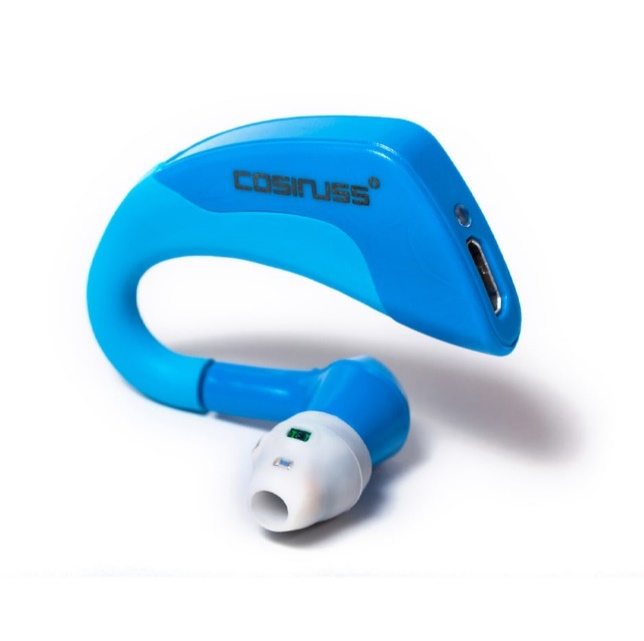
\includegraphics[scale=0.8]{figs/cosinuss}
   \caption{https://www.cosinuss.com/en/products/one}
   \label{fig:cosinuss}
\end{figure}


\subsection{Ballistocardiography}
BCG is the measurement of the mechanical effects of the beating heart on the body over time. Typically accelerometers or pressure sensors will be used to measure movement or forces on the surface of the body. BCG has been researched for use in ear heart rate extraction.

\medskip
In a wearable device proposed by \cite{da2010ear}, mechanical vibrations associated with heart rate are converted to electronic signals through capacitive sensing electrodes placed behind the ear. This method works by measuring the change in capacitance between the two electrodes as the distance between them changes due to heart rate vibrations.

\medskip
A study by \cite{winokur2012wearable} proposed measuring the head-to-foot axis recoil due to the blood-volume shift during cardiac ejection. This is done by placing an MEMS accelerometer behind the auricle. Due to the movement dependent method of operation this technology is extremely susceptible to motion artefacts and it can only be used during which the body is stationary.

\medskip
A variation of this technology is discussed in a article by \cite{park2015wearable}. They propose using a scissor shaped hinge mechanism in the ear canal that measures the change in the canal size due to the in-ear blood pulse waves. The mechanical movement is converted to an electrical signal through a piezoelectric film sensor. Figure \ref{fig:BCGsensor} shows an drawing of this device from Park's 2015 article.

\begin{figure}[h]
   \centering
   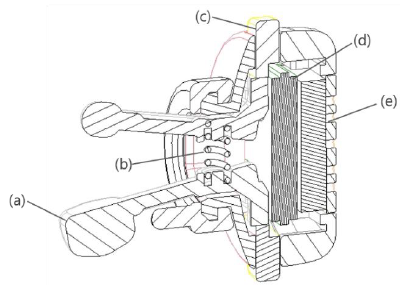
\includegraphics[scale=0.8]{figs/BCGsensor}
   \caption{Device to measure in ear pulse waves due to the heart beat \citep{park2015wearable}}
   \label{fig:BCGsensor}
\end{figure}

\subsection{Other Heart Rate Methods}
Electronic stethoscopes uses an microphone to record heart sounds. The hears makes a distinct series of sounds during the cardiac cycle due to blood turbulence and the shutting of heart valves. The period of this sound series can be used to determine heart rate and does not require skin-contact.

\medskip
A Doppler flow-meter can be used to detect the alternating blood current component in near-surface arteries. This component is synchronised to the heart rate frequency. The device can use ultrasound, microwaves of light to achieve the Doppler shift.

\section{Respiratory Rate}
Unlike the other medical signs, a person cannot measure his or her own respiratory rate. As soon as a person is consciously thinking about respiration, breathing usually slows. Measuring needs to happen while the person's thoughts are otherwise occupied. Therefore, a continuous measuring method are preferred. Typically, a nasal mask or chest strap will be used to measure respiration. 

\subsection{Ear Respiratory Rate Sensors}
Ear located devices that extract respiration information are rare, but some literature sources are available.

\medskip
\cite{goverdovsky2016hearables} tested an ear probe with two embedded microphones. The microphones could detect the sound created by turbulence in the airways for breathing rates higher than 12 breaths per minute. Figure \ref{fig:BreathingSound} shows a plot of the normalised sound amplitude at two different breathing rates. Variation during breathing can be seen in both recordings.

\begin{figure}[h]
   \centering
   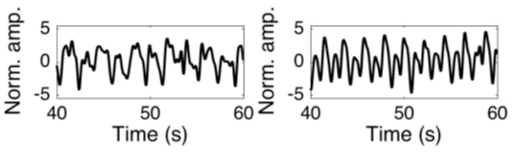
\includegraphics[scale=0.8]{figs/BreathingSound}
   \caption{Breathing detected through microphones inside the ear canal \citep{goverdovsky2016hearables}}
   \label{fig:BreathingSound}
\end{figure}

\cite{da2010ear} did extensive research on the ear as a location for medical sign monitoring. They extracted respiratory rate from baseline oscillations in a BCG signal recorded by capacitive electrodes placed behind the ear. Mechanical movement is converted to electrical signals by these electrodes. Therefore, the movement of the head due to respiration is seen on the BCG as baseline oscillations, Figure \ref{fig:BCGbreathing}.

\begin{figure}[h]
   \centering
   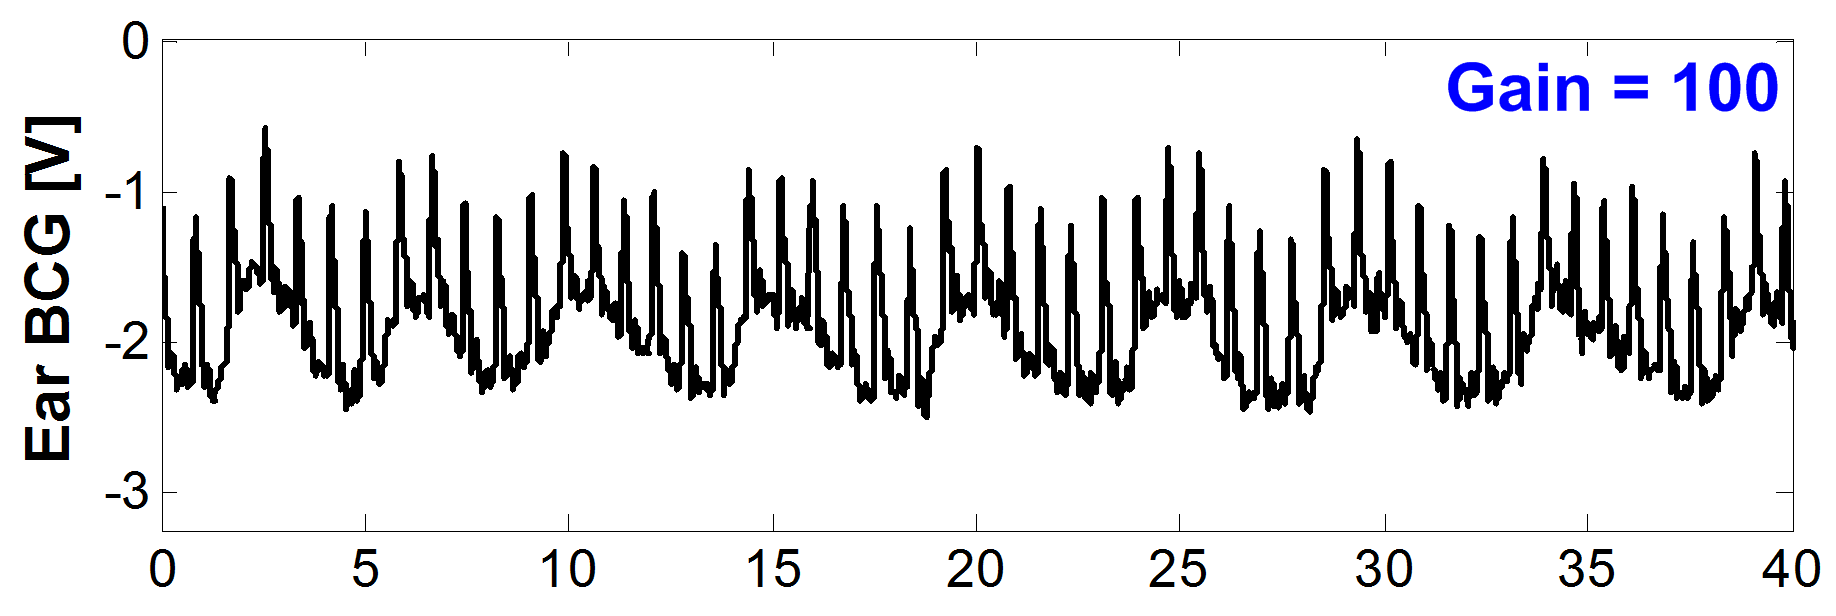
\includegraphics[scale=0.3]{figs/BCGbreathing}
   \caption{Baseline osculations in behind the ear BCG due to breathing \citep{da2010ear}}
   \label{fig:BCGbreathing}
\end{figure}

\subsection{Respiratory Related Heart Rate Characteristics}
A different approach is to extract respiratory rate by looking at the heart rate. A PPG signal contains three distinct respiratory related characteristics: amplitude modulation (AM), respiratory-induced intensity variation (RIIV) and frequency modulation \citep{johansson2003neural}.

\medskip
Amplitude modulation is due to blood pressure changes during the respiratory cycle called Pulsus Paradoxus. RIIV is chances in the volume of the dermis and subcutaneous capillary bed. It is visible as baseline variation in the PPG signal.  Frequency modulation of the heart rate synchronised to respiration rate, called respiratory sinus arrhythmia (RSA).

\medskip
RSA can also be detected in ECG, but differ from the fluctuations seen in chest ECG, due to electrodes movement relative to the heart and changes in chest impedance during the respiratory cycle \citep{moody1986clinical}. These fluctuations cannot be detected in the ear. RSA is observed as baseline oscillation in heart rate in synchrony with the respiratory rate. Heart rate increase during inspiration and a decrease during expiration \citep{yasuma2004_RSA}. According to a study done by \cite{stratton2003effects}, the variation in heart rate due to RSA is higher in younger test subjects with 74\% increase in children vs. 52\% increase in adults.

\medskip
Research was been done to develop algorithms to utilise these characteristics to extract respiratory rate from PPG signals. \cite{clifton2007measurement} used wavelet analysis, achieved a respiratory rate accurate to within 1 breath per minute and \cite{leonard2006fully} documented a respiratory rate error of 7.9\%. \cite{johansson2003neural} developed two neural network algorithms that uses the different respiratory related characteristics of PPG signals to detect breaths. Table \ref{table:RRC} shows the results of the best algorithm.

\begin{table}
\centering
\caption{Results of the respiratory rate extraction through neural networks \citep{johansson2003neural}}
\begin{tabular}{P{5cm}P{3cm}P{3cm}}
 \hline
 Respiratory Related Characteristics & False Positive (\%) & False Negative (\%) \\ 
 \hline
 RSA  	& 	3.7 	& 	6.9 \\  
 AM 	& 	5.2 	& 	4.7 \\
 RIIV 	&	5.2		&	5.9 \\
 \hline
\end{tabular}
\label{table:RRC}
\end{table}


\section{Blood Oxygen Saturation}
Oxygen saturation can be measured by means of an arterial blood gas test resulting an arterial oxygen saturation reading. This requires drawing a blood sample for testing and therefore is not relevant to this study. An alternative method is pulse oximetry. This method estimates peripheral capillary oxygen saturation, $SpO_2$, through the spectrophotometric analysis of PPG signals captured at two different wavelengths. This is a clinically excepted estimation of the arterial oxygen saturation.

\subsection{Pulse Oximetry Theory}
Blood oxygen saturation estimation through pulse oximetry relies on the different adsorption spectra of oxyhaemoglobin and deoxyhaemoglobin. Figure \ref{fig:AbsorptionSpectra} shows the absorption spectra of oxy- and deoxyhaemoglobin. 

\medskip
\begin{figure}
   \centering
   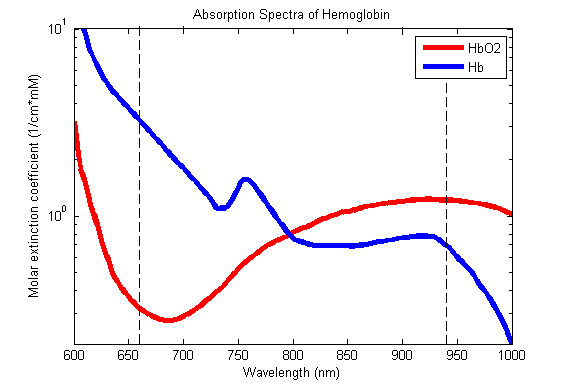
\includegraphics[scale=0.8]{figs/AbsorptionSpectra_Edit}
   \caption{Absorption spectra of oxy- and deoxyhemoglobin}
   \label{fig:AbsorptionSpectra}
\end{figure}

It can be noted that deoxyhaemoglobin has a significantly higher absorption of red light while oxyhaemoglobin has a slightly higher absorption of infrared light.

\medskip
According to Beers law, the amount of light absorbed by a dissolved substance is proportional to its concentration \citep{lambertANDbeer}. Therefore, oxygenated blood (with a higher concentration of oxyhaemoglobin) will absorb more infrared light and reflect more red light. Whereas deoxygenated blood (with a higher concentration of deoxyhaemoglobin) will absorb more red light and reflect more infrared light. This explains why oxygenated blood appears bright red, while deoxygenated blood is a darker shade of red.

\medskip
Red and infrared light are shined into the peripheral tissue and the light reflected or transmitted is measured for both wavelengths. Literature and commercial devices usually uses wavelengths of 660 nm (red) and 940 nm (near infrared) \citep{tytler1986nellcor} \citep{ti2012datasheet} \citep{bagha2011real} \citep{bheema2013spo2} \citep{duun2007novel}. The ratio of reflected or transmitted light is unique to a certain level of blood oxygen saturation and is used to estimate blood oxygen saturation.

\medskip
The Beer-Lambert law describes the absorption of a specific wavelength of light by a substance in a homogeneous solution \citep{bagha2011real}. 

$$A=\varepsilon cL=ln\left( \frac{I_o}{I}\right) $$
$$I=I_o e^{-\varepsilon _\lambda cL}$$

\medskip
Where $A$ is the dimensionless adsorption, $\varepsilon$ is the wavelength dependant molar absorptivity, $c$ is the concentration of the substance and $L$ is the path length the light needs to travel through the substance. $I_o$ is the intensity of the light entering the solution and $I$ is the intensity of light passing though the solution.

\medskip
When applying this law to measuring $O_2$ saturation, a concentration ratio can be calculated. Factoring out $L$, $I_o$, and the constants in $\varepsilon$, the ration can be written as:

$$R=\frac{log\left( I_{red} \right)\cdot\lambda _{red}}{log\left( I_{ir} \right)\cdot\lambda _{ir}}$$

\medskip
Where $I$ is the light intensities and $\lambda$ is the wavelength \citep{ti2012datasheet}.  Red and infrared light sources are alternated and intensity measurements are made for both separately.

\medskip
In practice, a different modulated relationship is used to compensate for the different DC absorption between patients \citep{konig1998reflectance} \citep{duun2007novel} \citep{bheema2013spo2}   \citep{bagha2011real}  \citep{nitzan2014calibration} \citep{ti2012application}

$$R = \frac{\left(\frac{AC}{DC}\right)\textsubscript{red}}{\left(\frac{AC}{DC}\right)\textsubscript{IR}} $$

\medskip
This ensures that the $O_2$ saturation of only the arterial blood is calculated. The ration can be checked against an empirical determined curve. The standard formula for this curve is found in literature as \% $SpO_2  = 110-25R$, \citep{ti2012application} but it can vary from device to device.

\medskip
As mentioned, $SpO_2$ can be calculated using reflected or transmitted light. Light that is not absorbed or scattered by tissue can be either reflected, or transmitted. Thus, both reflected and transmitted light is proportional to the mount of light absorbed. Transmittance mode pulse oximeters are more common, but their use is restricted to parts of the body that will allow for light to pass through, like a fingertip or earlobe.

\medskip
A big challenge to conventional pulse oximeters is noise due to movement \citep{spo2Motion}.

\subsection{Work done by others in ear pulse oximetry}
Standard locations for pulse oximetry includes the fingertip, earlobe, ankle and forehead. A study comparing fingertip and earlobe pulse oximetry to an arterial blood gas test found that finger pulse oximetry differed by a mean of -0,71\% and earlobe pulse oximetry differed by a mean of +4.2\% \citep{olive2016comparison}. Literature and commercial wearable pulse oximeters typically utilise a finger clip to measuring $SpO_2$ \citep{watthanawisuth2010wireless} \citep{pujary2003photodetector} \citep{huang2014novel} \citep{khalifa2014development}. This location is not ideal for continuous monitoring and is especially susceptible to motion artefacts. Although the fingertip location is not of interest to this study, the literature is still reviewed for similar principals can be applies to ear pulse oximetry.

\medskip
Ear lobe pulse oximetry usually done through a sensor that clips to the ear lobe, which is attached to a stationary device. Wearable ear pulse oximetry, is still novel and not well covered in literature. There are some patients filled for such devices (US 20050177034 A1) (US 4086915 A) (US 3412729 A) (US 6556852 B1) and commercial devices like but little academic material is available.

\medskip
A study done by \citep{aziz2006pervasive} tested a wireless earlobe-mounted pulse oximeter on a group of subjects. Subjects were tested while sitting, walking and running. During the sitting and walking phases they recorded an SpO2 reading of above 95\%, which is \enquote{as expected} according to them. But during the running phase they could not obtain any accurate reading. 

\medskip
During running, they could not take an $SpO_2$ reading, but Literature on ear PPG, only uses infrared light to determine heart rate. Theoretically, infrared light can be added in the same way to produce and red PPG and a R value can be calculated to estimate $SpO_2$.

\medskip
Pulse oximetry patch

\section{Electrical Brain Activity}

\chapter{Concept Design}
\label{chp:ConceptDesign}
This chapter builds upon the knowledge gained in the literature review and explains the logic used to select the methods and sensors to realize each medical sign monitoring requirement of the Ear-Monitor. Selections will be made by analysing advantages and disadvantages of each option and combining it with sound engineering judgement.

\section{Temperature}
The Ear-Monitor will measure core temperature from the inside of the ear canal. The main criteria are sensor size and measurement accuracy. The method- and sensor selection are discussed separately.

\subsection{Temperature measurement method}
Two temperature measuring methods are considered, namely contact- and non-contact thermometers.

\subsubsection{Contact thermometers}
A contact RTD, thermocouple or thermistor is placed in contact with the canal wall, canal air or tympanic membrane. Table \ref{tab:ContactThermometers_Eval} summarises the evaluation.

\begin{table}[H]
\caption{Contact thermometers evaluation}
\label{tab:ContactThermometers_Eval}
\renewcommand{\arraystretch}{1.3}	%Wat doen hierdie?
\centering
\begin{tabular}{|p{5cm}|p{8cm}|} 
 \hline
 Image 						& 	Advantages\\ 
							&	\tabitem Available in small sizes, ideal for the size restrictions of the ear canal.\\
  							&	\tabitem Good accuracy.\\
  							&	\tabitem Converting transducer voltage to temperature is simpler than with non-contact thermometers.\\
\hline
Sensor size: 0.5$\times$2.3 mm				& 	Disadvantages\\ 
Measurement accuracy: 0.15 $^{\circ}C$ 		&	\tabitem Canal wall and canal air temperature measurements can easily be influenced by ambient temperature conditions.\\
  											&	\tabitem Tympanic membrane contact can cause discomfort and harm to the wearer.\\
  											&	\tabitem More time is needed to take measurements, for the sensor needs to be in thermal equilibrium with the object.\\
 \hline
\end{tabular}
\end{table}

\subsubsection{Non-contact Thermometers}
A non-contact, infrared (IR) sensor is placed inside the ear canal and pointed at the tympanic membrane. Table \ref{tab:NonContactThermometers_Eval} summarises the evaluation.

\begin{table}[H]
\caption{Non-contact thermometers evaluation}
\label{tab:NonContactThermometers_Eval}
\renewcommand{\arraystretch}{1.3}	%Wat doen hierdie?
\centering
\begin{tabular}{|p{5cm}|p{8cm}|} 
 \hline
 Image 	& 	Advantages  \\ 
		&	\tabitem The sensor can measure the temperature of the tympanic membrane directly, which is the best representation of core temperature in the ear.\\
  		&	\tabitem Temperature conversion compensates for different ambient temperature conditions.\\
  		&	\tabitem No contact with the tympanic membrane lowers the injury risk to the user significantly.\\
\hline
Sensor size: 1.6 - 4 mm ${\diameter}$			&	Disadvantages  \\ 
Measurement accuracy: 0.2 - 0.5  $^{\circ}C$ 	&	\tabitem Non-contact temperature sensors are typically bigger than contact thermometers, adding to the size limitation challenge.\\
  												&	\tabitem If the tympanic membrane does not fill a considerable fraction of the sensor's field of view, erroneous measurements can occur.\\
 
 \hline
\end{tabular}
\end{table}

\subsubsection{Temperature measurement method choice}
A non-contact, IR sensor is selected for the Ear-Monitor. User safety, without significant performance compromise gives it superiority over contact thermometers for this application. The lower accuracy is justified by the fact that the tympanic membrane is a better representation of the core body temperature.

\subsection{Temperature measurement sensor}
To realize non-contact temperature measurement, two IR sensors are considered: The TMP006 from Texas Instruments and the ST60 Micro from Dexter Research Center Inc.

\subsubsection{ST60 Micro}
The ST60 Micro is a one channel, 80-junction, completely analogue temperature sensing device. It is enclosed in a Micro-TO package which is 4.09 mm in diameter as shown in Figure \ref{fig:ST60Micro}. The manufacturer emphasizes the ST60 Micro's versatility and proposes use in tympanic ear thermometers. A die temperature thermistor is available for ambient temperature compensation. Four wire are used to supply the sensor with power and to read transduced voltages.

 \begin{figure}[h]
   \centering
   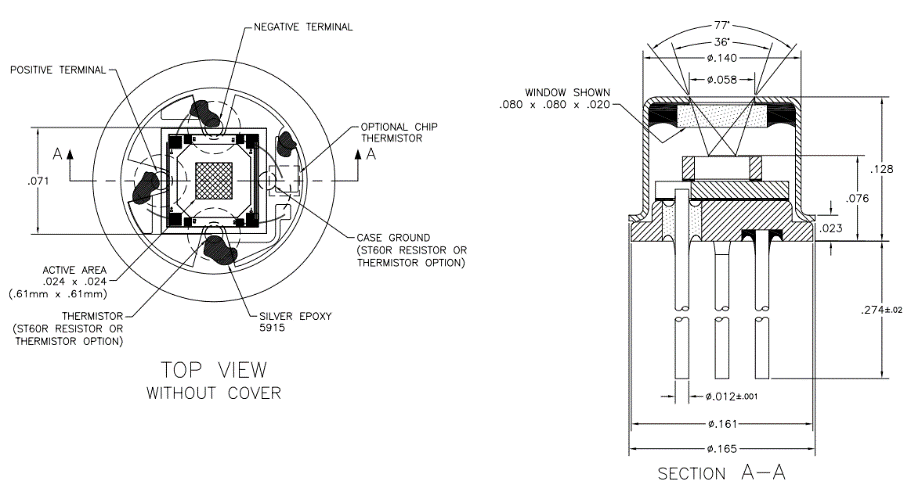
\includegraphics[scale=1]{figs/ST60Micro.png}
   \caption{ST60Micro diagram from the datasheet}
   \label{fig:ST60Micro}
\end{figure}

\subsubsection{TMP006}
The TMP006 is a fully integrated IR sensor measuring only 1.6$\times$1.6$\times$0.8 mm, ideally suited for a narrow ear canal. Thermophile voltage and sensor temperature, are made digitally available through hardware registers. These two values can be used to calculate the object temperature. Registers are accessed by a MCU though I\textsuperscript{2}C communication. Values are digitalized by a 16-bit on-chip ADC, eliminating the need for supporting analogue filters and amplifiers.
The TMP006's user guide suggest that is be used to calculate the surface temperature of target objects with emissivity values greater than 0.7, and preferably greater than 0.9. The literature study revealed that the emissivity of the eardrum is 0.98, placing it well within the required range.

\subsubsection{Temperature measurement sensor choice}
The simple shape of the ST60 Micro makes it easy to mount, but the diameter of the package may not fit in smaller ear canals and leave little room for the other sensors. Therefore, the ST60 Micro is eliminated.

\medskip

The smaller package size and on-chip ADC justifies the selection of the TMP006 for use in the Ear-Monitor. The TMP006 needs no separate analogue filter and amplifier. Furthermore, the manufacturer supplies detailed calibration documentation, allowing for more accurate and time effective calibration.

\section{Heart Rate}
The Ear-Monitor will extract heart rate from in or around the ear canal. The main criteria are sensor size, unobtrusiveness and the signal's susceptibility to noise. The method- and sensor selection are discussed separately. 

\subsection{Heart rate measurement method}

The following five methods from literature are considered to measure heart rate.

\subsubsection{Ear ECG}

As shown by \cite{winokur2012wearable}, an electrocardiogram can be detected behind the ear. One electrode is placed behind the ear on the mastoid bone and the other on the back of the neck. A differential amplifier and ADC is used to acquire the signal. Table \ref{tab:EarECG_Eval} summarises the evaluation.

\begin{table}[H]
\caption{Ear ECG}
\label{tab:EarECG_Eval}
\renewcommand{\arraystretch}{1.3}	%Wat doen hierdie?
\centering
\begin{tabular}{|p{5cm}|p{8cm}|} 
 \hline
 Image 						& 	Advantages  \\ 
  							&	\tabitem ECG is the standard method used by cardiologists to measure heart rate.\\
  							&	\tabitem Other cardiac information can be extracted from ECG i.e. heart rhythm, heart damage and the state of the conductive heart tissue.\\
  							&	\tabitem Not pulse transit time delay.\\
\hline
Sensor size: 10 mm  ${\diameter}$ electrodes					&	Disadvantages  \\ 
Unobtrusiveness: Bad - electrode needed behind ear and on neck 	&	\tabitem The sensor cannot be fitted entirely inside the ear canal.\\
Signal robustness: Noisy (Figure Winokur). 						&	\tabitem Two electrodes will be needed.\\
  																&	\tabitem Separate signal acquisition electronics are needed.\\
 
 \hline
\end{tabular}
\end{table}

\subsubsection{Ear PPG}
A LED and photodiode are used to detect variation in subcutaneous tissue blood volume due to the beating heart. Literature identifies three possible locations: Inside the ear canal, the earlobe and the concha. With unobtrusiveness in mind, the ear canal method is selected. This means reflective PPG is used. Table \ref{tab:EarPPG_Eval} summarises the evaluation.

\begin{table}[H]
\caption{Ear PPG}
\label{tab:EarPPG_Eval}
\renewcommand{\arraystretch}{1.3}	%Wat doen hierdie?
\centering
\begin{tabular}{|p{5cm}|p{8cm}|} 
 \hline
 Image 		& 	Advantages  \\ 
  			&	\tabitem A substantial pressure pulse can be detected in and around the ear.\\
  			&	\tabitem Pulse oximetry, a type of PPG, is a tried and tested way of measuring heart rate and SpO\textsubscript{2}.\\
  			&	\tabitem Respiratory related characteristics like amplitude modulation, respiratory-induced intensity variation and frequency modulation can be found only in PPG signals and can be used to determine respiratory rate.\\
\hline
Sensor size: Smallest - 1.9$\times$2.6$\times$0.8 mm		&	Disadvantages  \\ 
Unobtrusiveness: Good - fits inside ear canal 				&	\tabitem PPG is susceptible to motion artefacts and variation in blood profusion.\\
Signal noise: Low - clear pressure wave visible (Figure da2010ear) 						&	\tabitem Few PPG sensor packages are available to fit inside the ear canal.\\
  															&	\tabitem Using separate LEDs and photo detectors increases the complexity  and size for the proof of concept Ear-Monitor.\\
 
 \hline
\end{tabular}
\end{table}

\subsubsection{Ear BCG}
A pressure sensitive sensor or accelerometer is placed inside the ear canal to detect the mechanical effects of the pulsating heart. Table \ref{tab:EarBCG_Eval} summarises the evaluation.

\begin{table}[H]
\caption{Ear BCG}
\label{tab:EarBCG_Eval}
\renewcommand{\arraystretch}{1.3}	%Wat doen hierdie?
\centering
\begin{tabular}{|p{5cm}|p{8cm}|} 
 \hline
 Image 		& 	Advantages  \\ 
  			&	\tabitem Pressure sensors can be made small enough for the limited space in the ear canal.\\
  			&	\tabitem Accelerometer can also be used to measure respiratory rate.\\
\hline
Sensor size: Smallest - 3$\times$3$\times$1 mm	[3]									&	Disadvantages  \\ 
Unobtrusiveness: A part of the sensor protrudes from the ear, can be made smaller 	&	\tabitem The signal detected by \cite{da2010ear} and \cite{winokur2012wearable} appears noisy and detecting beats will be troublesome.\\
Signal noise: High (da2010ear) (winokur2012wearable) 							&	\tabitem This method will be influenced by motion artefacts to such an extent that it will be unusable for most forms of practical use.\\
 
 \hline
\end{tabular}
\end{table}

\subsubsection{Phonocardiogram}
A microphone is placed inside the ear canal and identifies heart beats by analysing the sound produced by the cardiac cycle. Table \ref{tab:EarPhonocardiogram_Eval} summarises the evaluation.

\begin{table}[H]
\caption{Ear Phonocardiogram}
\label{tab:EarPhonocardiogram_Eval}
\renewcommand{\arraystretch}{1.3}	%Wat doen hierdie?
\centering
\begin{tabular}{|p{5cm}|p{8cm}|} 
 \hline
 Image 		& 	Advantages  \\ 
  			&	\tabitem Can be used to detect breathing as well, as shown by \cite{goverdovsky2016hearables}.\\
\hline
Sensor size: Smallest - 3.35$\times$2.5$\times$0.98 mm	&	Disadvantages  \\ 
Unobtrusiveness: Can fit inside the canal [5]			&	\tabitem Sounds from other sources like movement and speaking can corrupt the signal.\\
Signal noise: High 								&	\\
 
 \hline
\end{tabular}
\end{table}

\subsubsection{Heart rate method choice}
Ear PPG is selected as the Ear-Monitor's method of measuring heart rate. PPG produces a clear signal that will allow for accurate beat detection. This method can also be in cooperated into the $SpO_2$ measurement sensor, eliminating the need for two different sensors. The entire sensor can fit inside the ear canal making it unobtrusive. This method is also less susceptible to noise than ear BCG or a phonocardiogram.

\subsection{Heart rate measurement sensor}
Reflexive ear canal PPG is selected to measure heart rate. Three PPG sensors options are considered namely: separate LEDs and photodetector, the NJL5501R from JRC and the MAX30100 by Maxum Integrated.

\subsubsection{Separate LEDs and photodetector}
SMD LEDs is used along with one or more photo detectors. The components are mounted on a thin PCB and placed in the ear probe. The LEDs and photo detectors can be placed in various precise configurations and a wider choice of individual transducers can be used. Additional analogue electronics are needed to drive the LEDs, conditioning the detector signal output and compensate for ambient lighting. A commercial integrated analogue front end chip like Texas Instruments' AFE4400 can be used to perform this task.

\subsubsection{NJL5501R}
The NJL5501R is a surface mounted photo-emitter and -detector contained in one 1.9$\times$2.6$\times$0.8 mm package shown in Figure \ref{fig:NJL5501R}. Red and IR LEDs make it suitable for reflective pulse oximetry and heart beat detection. Its small size will allow it to fit in the ear canal while leaving adequate space for other sensors. It requires all the same supporting electronics as using the separate LEDs and a photo-detector method.

 \begin{figure}[h]
   \centering
   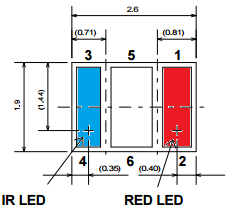
\includegraphics[scale=1]{figs/NJL5501R.png}
   \caption{NJL5501R diagram from the datasheet}
   \label{fig:NJL5501R}
\end{figure}

\subsubsection{MAX30100} 
The MAX30100 is single chip pulse oximeter and heart rate detector. It has red and IR LEDs, a photodetector, a 16-bit ADC and digital filters all in one 5.6$\times$2.8$\times$1.2 mm, 14-Pin package. The LEDs and photodetector are in the same plane, meaning it operates in reflective mode. Like the TMP006 is uses the I2C protocol to communicate with a MCU. Configuration registers allow the designer to specify sample rate, LED currents and LED pulse width. Figure \ref{fig:MAX30100_Diagram} shows a block diagram of the internal systems of the MAX30100.

\begin{figure}[H]
   \centering
   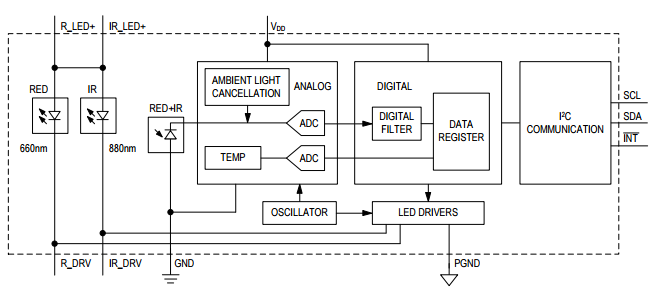
\includegraphics[scale=1]{figs/MAX30100_Diagram.png}
   \caption{MAX30100 block diagram from the datasheet}
   \label{fig:MAX30100_Diagram}
\end{figure}

The MAX30100 uses a 3.3V supply and programmable current sources to drive the LEDs, whilst digital operations are done at 1.8V. It draws between 6 and 12 mA while recording red and IR PPGs. It has a digital 50Hz/60Hz notch filter to reject powerline interference. LEDs can be individually supplied with 0 mA to 50 mA and LED pulse width can be varied from 0.2 ms to 1.6 ms. A sample rate can be chosen between 5 and 1000 samples per second. An important feature of the MAX30100 is its 64-byte deep FIFO register which is used to store the output values. Each output set consists of a 16-bit red and 16-bit IR value, meaning that there are 4 bytes per output and therefore 16 sets of output values can be held in the FIFO art any time. The MCU will read 4 bytes at a time from the FIFO to obtain the latest red and IR values.

\subsubsection{Heart rate sensor choice}
The MAX30100 is selected for use in the Ear-Monitor. It has optimized optics to guide outgoing and incoming light. It has integrated ambient light cancellation. Its entire AFE is integrated meaning that no additional electronics are needed, apart from the I2C lines and power regulators. This gives if a big advantage over the more complex separate LEDs and photodetector method. Its small size and reflective mode of operation, allows it to be placed inside of the ear canal. Data recorded by the MAX30100 will be used to calculate heart rate and SpO\textsubscript{2}. 

\section{Respiratory Rate}
The Ear-Monitor will measure respiratory rate from inside the ear canal. The main criteria are sensor size and susceptibility to noise corruption.

\subsection{Respiratory rate measuring method}
The following three respiratory rate measuring methods from literature are considered.

\subsubsection{Accelerometer}
A small MEMS accelerometer is placed inside the ear canal and measures the movement of the head due to breathing. Table \ref{tab:EarAccelerometer_Eval} summarises the evaluation.

\begin{table}[H]
\caption{Ear Accelerometer}
\label{tab:EarAccelerometer_Eval}
\renewcommand{\arraystretch}{1.3}	%Wat doen hierdie?
\centering
\begin{tabular}{|p{5cm}|p{8cm}|} 
 \hline
 Image 		& 	Advantages  \\ 
  			&	\tabitem The accelerometer can serve the dual purpose of measuring breathing and heart rate, thus saving space.\\
\hline
Sensor size: 3$\times$3$\times$1 mm	[3]					&	Disadvantages  \\ 
Noise: Very high							&	\tabitem This method is extremely vulnerable to noise form other movements.\\
 \hline
\end{tabular}
\end{table}

\subsubsection{Microphone}
A microphone is placed inside the ear canal and record the sound of air moving through the respiratory tracts, allowing the respiratory rate to be determined. Table \ref{tab:EarMicrophone_Eval} summarises the evaluation.

\begin{table}[H]
\caption{Ear Microphone}
\label{tab:EarMicrophone_Eval}
\renewcommand{\arraystretch}{1.3}	%Wat doen hierdie?
\centering
\begin{tabular}{|p{5cm}|p{8cm}|} 
 \hline
 Image 		& 	Advantages  \\ 
  			&	\tabitem The microphone can serve the dual purpose of measuring breathing and heart rate, thus saving space.\\
\hline
Sensor size: ?					&	Disadvantages  \\ 
Noise: Very high	&	\tabitem This method is extremely vulnerable to noise form other sounds like talking or ambient noise.\\
 \hline
\end{tabular}
\end{table}

\subsubsection{Respiratory related heart rate characteristics}
The variations in heart rate is used to determine the respiratory rate. These include amplitude modulation, respiratory-induced intensity variation and frequency modulation of the heart rate in synchronization with the respiration rate. Table \ref{tab:EarRRHRC_Eval} summarises the evaluation.

\begin{table}[H]
\caption{Respiratory related heart rate characteristics}
\label{tab:EarRRHRC_Eval}
\renewcommand{\arraystretch}{1.3}	%Wat doen hierdie?
\centering
\begin{tabular}{|p{5cm}|p{8cm}|} 
 \hline
 Image 		& 	Advantages  \\ 
  			&	\tabitem No dedicated sensor is needed.\\
  			&	\tabitem Less susceptible to noise the accelerometer or microphone method.\\
\hline
Sensor size: No sensor needed		&	Disadvantages  \\ 
Noise susceptibility: Low			&	\tabitem Only steady and relatively slow respiratory rates can be detected.\\
 \hline
\end{tabular}
\end{table}

\subsubsection{Respiratory rate choice}
The Ear-Monitor will determine respiratory rate by analysing respiratory related heart rate characteristics, of which heart rate frequency modulation through respiratory sinus arrhythmia (RSA) is found to be the most detectable. This method saves space by not requiring a dedicated sensor. It is also the lest susceptible to noise from other sources. No sensor selection is needed for this medical sign, as all the work is done by the micro controller.

\section{Blood oxygen saturation}
Pulse oximetry is the only practical way for the Ear-Monitor to measure blood oxygen saturation. The MAX30100 selected for measuring heart rate is equipped for this task. A red and IR LED as well as a photo-detector is available for the joint function for measuring heart rate and SpO\textsubscript{2}.

\section{Final concept}
The final concept is obtained by combining the methods and sensors selected in this chapter. To summarise: the Ear-Monitor will used the TMP006 IR sensor pointed at the tympanic membrane to measure core body temperature. The MAX30100 reflective pulse oximeter will be placed on on the side of the ear probe facing the canal wall. Red and IR PPGs from the MAX30100 will be used to extract heart rate and SpO\textsubscript{2}. Finally, respiratory rate will be determined by analysing the respiratory sinus arrhythmia.

\medskip

Additionally, a multi controller unit (MCU), battery and wireless transceiver are selected for the Ear-Monitor. The Arduino Pro Mini MCU has the necessary I/O pins for serial communication with the sensors and wireless module. It is also easy to program, making it ideal for the proof of concept version of the Ear-Monitor. Lithium-ion batteries are currently the best choice while regarding capacity, compactness and price and is therefore selected to supply the power to the Ear-Monitor. Bluetooth is the typically used standard for transmitting data over short distances and is supported by most modern smart devices. The HC-05 Bluetooth modem is selected and will allow the Ear-Monitor to send data to a supporting device through a wireless connection. Figure \ref{ConceptDrawing} shows a diagram of the Ear-Monitor concept with a more detailed drawing of the ear probe with the selected sensors.

\begin{figure}[H]
   \centering
   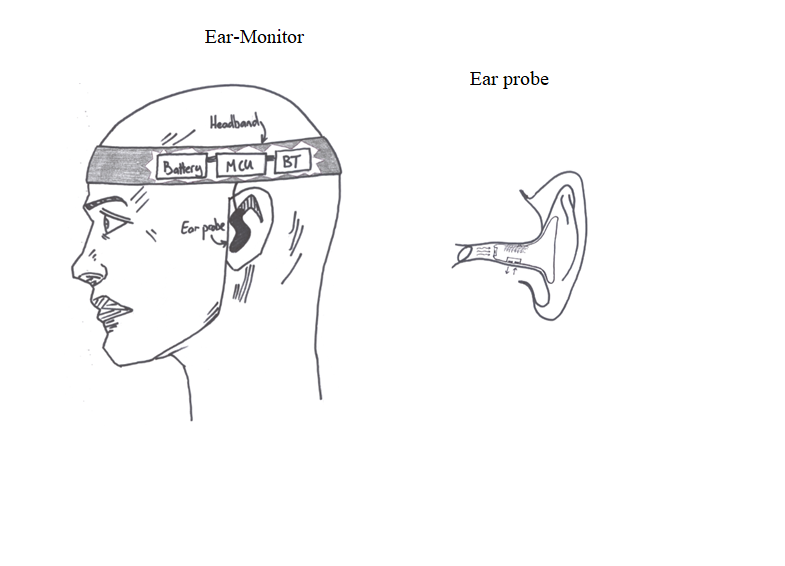
\includegraphics[scale=1]{figs/ConceptDrawing.png}
   \caption{Drawing of the selected Ear-Monitor concept and a more detailed drawing of the ear probe with sensors (Add labels)}
   \label{fig:ConceptDrawing}
\end{figure}

\chapter{Detailed Design}
\label{chp:DetailedDesign}
This chapter documents the detailed design of the Ear-Monitor's subsystems. The hardware and software sides are discussed separately. 

\section{Hardware}

A typical telemedicine configuration is used for the Ear-Monitor and its supporting system. It is similar to the configuration used by \cite{wang2010wearable} and \cite{prawiro2016integrated} for their respective wearable health monitors. The ear-probe is the signal acquisition module of the Ear-Monitor and contains the sensors. A microcontroller unit (MCU) is used to control the flow of data within the Ear-Monitor and data is sent by means of a wireless transceiver to a device running supporting software, where data is stored for later access. Figure \ref{fig:HardwareFlowchart} illustrates the flow of information through the hardware set-up.

\begin{figure}[h]
\centering
\graphicspath{{figs/}}
\input{figs/HardwareFlowchart.pdf_tex}
\caption{Flow of information in a typical telemedicine set-up}
\label{fig:HardwareFlowchart}
\end{figure}

This section documents the detailed design of each of the key parts of hardware found in the Ear-Monitor.

\subsection{Temperature sensor}
The non-contact, IR TMP006 is selected to measure tympanic membrane temperature in the Ear-Monitor. Four wires are connected for power and serial communication lines. The package has eight solder balls for surface mounting on a printed circuit board (PCB). A big challenge was to mount this micro-component. Various methods were tested:

\begin{itemize}
\item A PCB was designed and manufactured, but mounting the miniature TMP006 on this PCB proved to be problematic.
\item The device footprint and wire connection pads were etched into copper clad flexible circuit board sheets. Solder paste and a heat gun was used to mount the TMP006. This method worked, but mounting proved to be unreliable, for connections were sometimes not made properly or the TMP006 got damaged.
\item Pre-mounted boards were acquired and the excess material were cut away to allow wires to be soldered to the exposed tracks.
\end{itemize}

\medskip

This last method proved to be the best solution for the proof of concept version of the Ear-Monitor. It was necessitated by the lack of advanced facilities to mount micro SMT components. The flexible circuit board method will be preferable when a SMT component placement system is available. Figure \ref{fig:TMP006_Breakout} shows the bought, pre-mounted boards and the cut-out component along with the four connections. 3.3V and ground (GND) are connected to a power regulator and the two serial communication wires are connected to the serial communication I/O pins of the MCU.

\begin{figure}[h]
\centering
\graphicspath{{figs/}}
\input{figs/TMP006_Breakout.pdf_tex}
\caption{(a) TMP006 pre-mounted boards and (b) the cut-out sensor segment with four connections labeled}
\label{fig:TMP006_Breakout}
\end{figure}

According to the TMP006's user guide, the sensor captures radiation form almost its entire 180\textdegree{} field of view (FOV), but the majority of the received signal comes from sources that are parallel to, and precisely in front of the sensor. The final target object temperature is an integration of all the radiation signals captured across the FOV of the sensor.

\medskip

The user guide also states that the smaller the object is, the closer it should be placed to the sensor to prevent other objects from entering the field of vision. The goal is to place the sensor at least 5mm from the membrane. This will remove the risk of contact with the membrane, while still ensuring thermal radiation from the canal is detected. Energy from the ear canal self will inevitably be detected by the sensor, but the majority of the radiation will come from the membrane and it is assumed that the wall near the membrane is in thermal equilibrium with the membrane within an acceptable margin. To achieve this position, the TMP006 will be placed at the tip of the ear probe.

\medskip

Energy radiated or conducted between the PCB and the sensor can cause temperature calculation errors. To prevent this the sensor and PCB should be kept at the same temperature. The ear probe set-up of the Ear-Monitor is favourable for this task, for the PCB is very small and contains no other heat generating components. Also, the target object, tympanum, will stay at a constant temperature, so the sensor will experience no heat fluctuations. It will, however, be necessary to allow time for the sensor and PCB to reach thermal equilibrium once placed inside the ear canal, before accurate measurements can be taken. This will not be a problem, for the device is designed to be worn continuously for long periods of time.

\subsection{Pulse Oximeter}
The MAX30100 pulse oximeter is selected to record red and IR photoplethysmographs from inside the ear canal. These are used for determining heart rate and SpO\textsubscript{2}. The MAX30100 is controlled with 5 connection wires, connected to 7 of the package's 14 pins. Figure \ref{fig:MAX30100_pinout} shows a diagram of the MAX30100 package and the required connections for operation. 3.3 V, 1.8 V an GND are connected to a power regulator and the two serial communication lines are connected to the serial communication I/O pins of the MCU.

\begin{figure}[H]
\centering
\graphicspath{{figs/}}
\def\svgwidth{180pt}
\input{figs/MAX30100_pinout.pdf_tex}
\caption{MAX30100 package diagram with required connections for operation.}
\label{fig:MAX30100_pinout}
\end{figure}

As with the TMP006, the mounting of the extremely small MAX30100 was a great challenge. The first attempt was to design and manufacture a PCB on the typically used, 1.6 mm thick, FR4 PCB material. This PCB proved to be too thick and its inflexibility caused extra problems in ensuring firm contact with the ear canal wall. The solution was to etch the footprint, tracks and pads into flexible circuit board material. The etching process involves:
\begin{itemize}
\item Design the layout on EAGLE PCB open source software.
\item Print the mirrored layout on toner transfer paper.
\item Preparing the copper clad material by cleaning with rubbing alcohol.
\item Transfer the ink form the toner transfer paper to the copper clad material by applying heat and pressure.
\item Submerge the copper clad material with ink layout in ferric chloride (FeCL\textsubscript{3})
\item Cleaning off the remaining ink with acetone to reveal the copper tracks.
\end{itemize} 

The ferric chloride dissolves all the copper that is exposed, leaving copper tracks that were covered by the ink during etching. The flexible copper clad material is \SI{60}{\micro\meter} thick, making it ideal for the size limitations inside the ear canal. Figure \ref{fig:MAX30100_layout} shows the layout designed and resulting etched flexible circuit board. The flexible nature of the circuit board allows it to be folded in halve to form a two sided circuit board, saving space and placing the all connection pads on the same end. It also allows for uniform and firm contact between the MAX30100 and the ear canal wall. Wires for power and communication are soldered to the five connection pads.

\begin{figure}[H]
\centering
\graphicspath{{figs/}}
\def\svgwidth{180pt}
\input{figs/MAX30100_layout.pdf_tex}
\caption{(a) is the layout as designed on EAGLE PCB  with the outline of the MAX30100 shown in black and (b) is the finished flexible PCB with copper tracks (insert scale?)}
\label{fig:MAX30100_layout}
\end{figure}

\subsection{Control and Communication Hardware}
The remaining electronic components consisted of the Arduino MCU, HC-05 Bluetooth modem and battery. A PCB is designed to integrate all the the different hardware subsystems. Additional electronics include the power regulators, I\textsuperscript{2}C pull-up resistors and a charging circuit for the LiPo battery. A on-off switch and power-on indicator LED are also added. 

\medskip

\SI{10}{\kilo\ohm} pull-up resistors on the SDA and SCL lines are recommended for standard I\textsuperscript{2}C communication and are therefore included in the design. A \SI{7.4}{\volt}, \SI{1000}{\milli\ampere\hour} rechargeable LiPo battery (https://www.robotics.org.za/603450?search=battery) is selected to supply power to the Ear-Monitor. The Ear-Monitor will be operate for XXX minutes on a sigle charge (Calculations in Appendix Y). The Arduino has its own power regulation circuitry on board and can be connected directly to the battery. Two low drop-out voltage regulators are selected to supply 1.8 V and 3.3 V to the sensors and Bluetooth modem. A charging circuit is added to allow the battery to be charge without physically disconnecting it from the device. Decoupling capacitors are added to all power supply lines. Figure \ref{fig:Ear-Monitor_BlockDiagram} shows block diagram of the Ear-Monitor's hardware. The diagram is split between the components on the PCB worn on the hear and the components in the ear probe.

\begin{figure}[H]
   \centering
   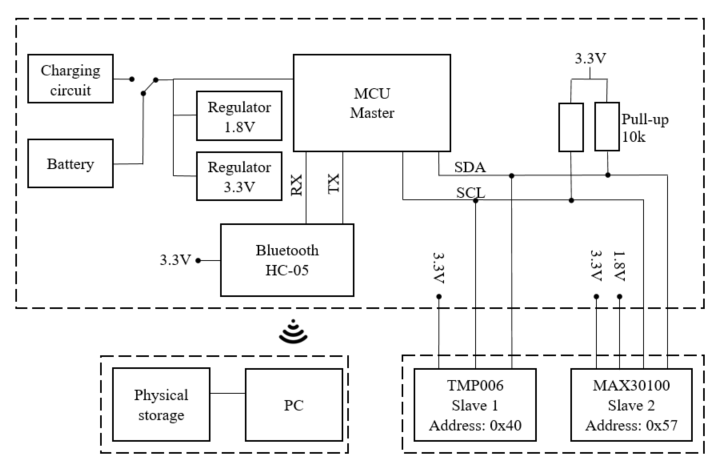
\includegraphics[scale=0.9]{figs/Ear-Monitor_BlockDiagram.png}
   \caption{Block digram for the Ear-Monitor's hardware components}
   \label{fig:Ear-Monitor_BlockDiagram}
\end{figure}

A schematic diagram and PCB layout is included in Appenxix (X). Calculations to select passive components is included in Appendix Y. The MCU, battery, Bluetooth modem and PCB will be worn in a headband around the head in this proof of concept version of the Ear-Monitor. Only the TMP006 and MAX30100 will be located at their correct positions in the ear canal hold in place by the ear probe. The ear probe is connected by a wire to the electronics in the headband. Data is sent from the headband to the PC through the wireless connection. It is well within the abilities of the current state of technology to reduces the size of all the electronics to a hearing aid, or even ear probe size device. But such miniaturisation is not within the scope of this project.

\medskip

An ear probe is designed to hold the MAX30100 and TMP006 in the correct positions in the ear canal and restrict their movement to minimize artefacts. Sugru\textsuperscript{\textregistered} is the band name for a mouldable silicone elastomer which is perfect for this application. According to the product documentation it is non-toxic and does not cause skin irritation. The mouldable putty is pressed into the ear and assumes the its shape, but does not conform completely, therefore allowing it to fit in different ear shapes. When cured, it has a sturdy, but flexible structure. Slots and holes are cut into the moulded probe to hold the sensors and wires. Figure \ref{fig:EarProbe} shows a photo of the completed ear probe.

\begin{figure}[H]
   \centering
   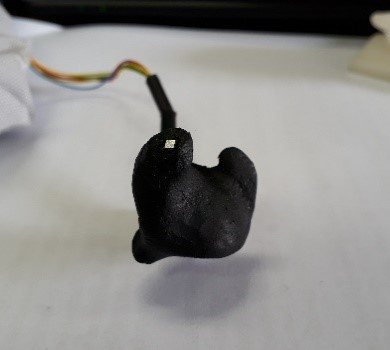
\includegraphics[scale=1]{figs/EarProbe.jpg}
   \caption{}
   \label{fig:EarProbe}
\end{figure}

Add a photo of the completed electronic hardware





\section{Software}
Software is written for the MCU and for the PC receiving and storing the data. MCU software is C++ based and developed using the Arduino IDE. MCU software handles sensor communication, timing, some processing and transmitting collected data via the Bluetooth modem. The PC software is Java based and developed using the Processing IDE. The PC software listens on the Bluetooth serial port, processes received data, display the data via a user interface and stores the received data on the local hard drive.

\medskip

Figure \ref{fig:Software_BlockDiagram} shows a diagram of the flow of data through the various software functions. The final calculated medical signs are shown in blue. The diagram is split between the MCU functions and PC functions. MCU and PC software are connected through the Bluetooth connection. The main functions are discussed in this section.

\begin{figure}[H]
   \centering
   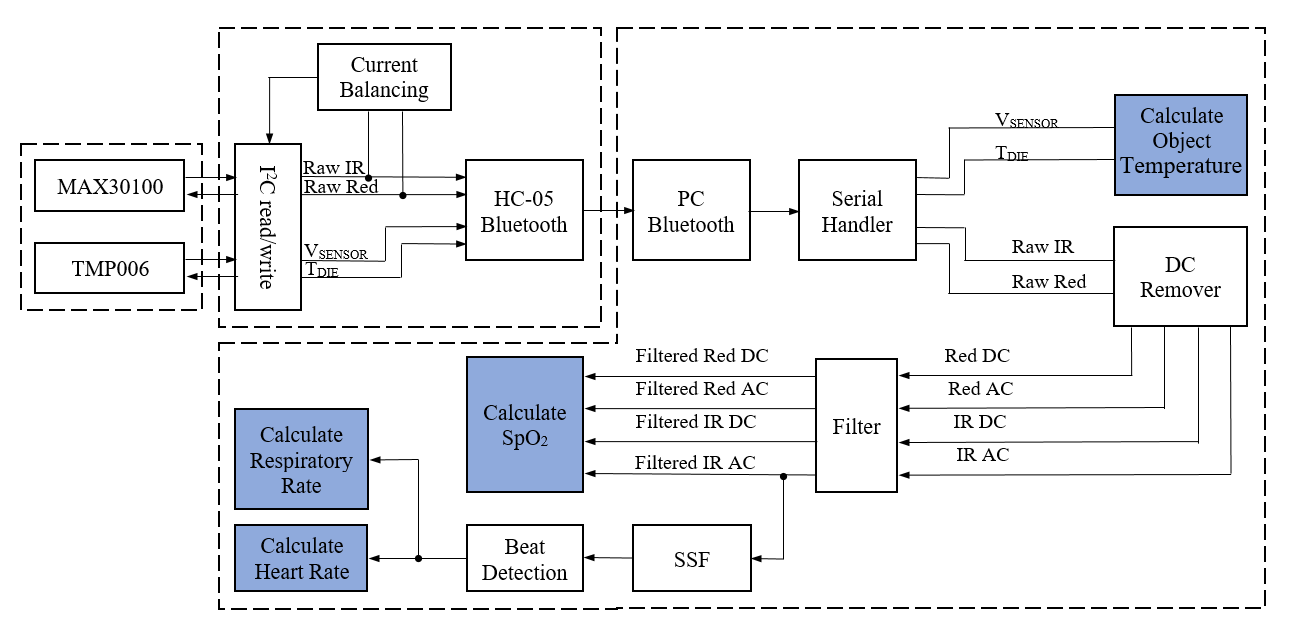
\includegraphics[scale=0.45]{figs/Software_BlockDiagram.png}
   \caption{Block diagram showing the flow of information through the various software functions. Final calculated medical signs are shown in 	blue}
   \label{fig:Software_BlockDiagram}
\end{figure}

\subsection{Sensor Communication Software}
Software is written for the MCU to communicate with the sensors and Bluetooth module. The MAX30100 and TMP006 have different default addresses and can share one I\textsuperscript{2}C bus for communication with the MCU. I\textsuperscript{2}C communication happens one byte at a time with no parity and MSB first. The eighth bit of the address indicates a read or write request. Figure \ref{fig:I2C_Read} shows how the software reads 16-bit values from the TMP006 registers. Values form the MAX30100 are read in a similar way.

\begin{figure}[H]
   \centering
   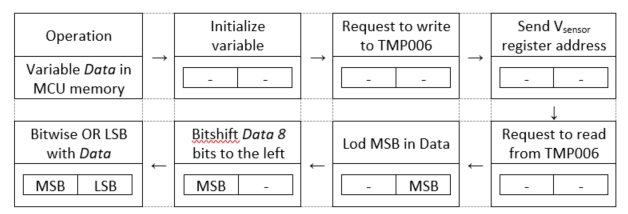
\includegraphics[scale=1]{figs/I2C_Read.png}
   \caption{How the software reads 16-bit values from the TMP006 registers}
   \label{fig:I2C_Read}
\end{figure}

Communication with sensors consists of two steps, configuration and reading data.

\subsubsection{Sensor Configuration}
Upon power on, both sensors start with default configurations. The MCU is programmed to reconfigure both sensors on start-up. This is done by writing values to the various configuration registers.
The MAX30100 is set to SpO\textsubscript{2} mode with \SI{1600}{\micro\second} LED pulse width, 50 Hz sampling rate and \SI{50}{\milli\ampere} current supply to both LEDs. The TMP006 is set to use the average of 16 conversions per output, meaning it will sample at 0.25 Hz. This is done, because the application does not demand a high sampling rate and increasing the number of samples per output will reducing noise (\SI{0.125}{\celsius}). These configurations are done every time the Ear-Monitor is powered on.

\subsubsection{Reading data from sensors}
After configuration is done, the MCU enters a continuous loop of sensor data reading. The MAX30100 uses one FIFO register to store the latest 16 IR and red photo-detector voltages and the TMP06 has two separate registers for die temperature and sensor voltage. These registers are red through Arduino's Wiring library. The MAX30100 outputs at 50 Hz and the TMP006 at 0.025 Hz. A timing loop is created to ensure that the values are red from the sensors in time.

\subsection{Temperature related software}
After start-up configuration, two values, V\textsubscript{SENSOR} and T\textsubscript{DIE}, are read from the TMP006 through the I\textsubscript{2}C connection every 4 seconds.

\medskip

T\textsubscript{DIE} is measured by an on-chip precision thermistor and digitalized to a 14-bit value in binary two's compliment, signed integer format with one LSB equal to \SI{0.03125}{\celsius}. After two bytes has been read from the TMP006's T\textsubscript{DIE} register (as shows in Figure \ref{fig:I2C_Read}), it is bitshifted twice to the right to get the 14-bit value and then divided by 32 to get the temperature in \SI{}{\celsius}. Table \ref{tab:Tdie_Example} show an example calculation to obtain T\textsubscript{DIE}. This conversion is done on the MCU and the value in \SI{}{\celsius} is transmitted over the Bluetooth connection.

\begin{table}[H]
\caption{T\textsubscript{DIE} example calculation}
\label{tab:Tdie_Example}
\renewcommand{\arraystretch}{1.3}
\centering
\begin{tabular}{|P{4cm}|P{4cm}|P{1.5cm}|P{2.5cm}|} 
\hline
Digital output			& 	Right shifted twice 	& 	Decimal 	& $\div$ 32\\
\hline
0000 1100 1000 0000		& 	0000 0011 0010 0000		& 	800 		& \SI{25}{\celsius}\\
\hline
\end{tabular}
\end{table}


V\textsubscript{SENSOR} is the output of the thermopile and ranges from -5.12 to \SI{5.12}{\milli\volt}. The 16-bit ADC converts this analogue value to a digital value with a LSB equal to $\frac{5.12-(-5.12)}{2^16}= \SI{156.25}{\nano\volt}$. Conversion to voltage is done prior to sending the voltage value over the Bluetooth connection.

\medskip

T\textsubscript{DIE} and V\textsubscript{SENSOR} are received by the PC software, where they are used to calculate T\textsubscript{OBJ}. One sensor voltage and die temperature conversion cycle takes \SI{250}{\milli\second}, and the device gives the designer an option to choose the number of conversions ($N$) per output sample. The average of the $N$ samples is loaded into the output register every $N\times\SI{250}{\milli\second}$. The this design $N$ is chosen to be 16 and the time per register output equals 4 seconds.

\subsection{Calculating T\textsubscript{OBJ}}
T\textsubscript{DIE} and V\textsubscript{SENSOR} are used to calculate T\textsubscript{OBJ}. The TMP006's datasheet suggests using the relationship:
\begin{equation}
\label{eq:TempCurve1}
	T_{OBJ} = \sqrt[4]{{T_{DIE}}^4-\frac{f(V_{SENSOR})}{S}}
\end{equation}
Where $f(V_{SENSOR})$ is a function that compensates for heat flow in the form of convection and conduction. The function is described in two stages by:
\begin{equation}
\label{eq:TempCurve2}
	V_{OS}=B0+B1(T_{DIE}-T_{REF})+B2(T_{DIE}-T_{REF})^2
\end{equation}
\begin{center}and\end{center}
%and
\begin{equation}
\label{eq:TempCurve3}
	f(V_{SENSOR}) = (V_{SENSOR}-V_{OS})+C(V_{SENSOR}-V_{OS})^2
\end{equation}
Where $V_{OS}$ is a compensating offset voltage, $T_{REF}$ is a reference temperature equal to \SI{25}{\celsius} and $B0$, $B1$, $B2$ and $C$ are calibration parameters.

\medskip

S takes into account the object emissivity ($\varepsilon$), Stefan-Boltzman constant ($\sigma$) and the non-ideal absorption of the sensor itself. It is described by:
\begin{equation}
\label{eq:TempCurve4}
	S=S0(1+A1(T_{DIE}-T_{REF})+A2(T_{DIE}-T_{REF})^2
\end{equation}
Where $S0 = \varepsilon\sigma$, $T_{REF}=\SI{25}{\celsius}$ and $A1$ and $A2$ are parameters experimentally derived through calibration.

\medskip

The TMP007 is the same sensor as the TMP006, but with a built in math engine. The recommended calibration parameters from the TMP007's data sheet is shown in Table \ref{tab:Calibration_Vals}. This parameters can also be seen as the default calibration parameters for the TMP006 and is a good starting point for the calibration process.

\begin{table}[H]
\caption{T\textsubscript{DIE} example calculation}
\label{tab:Calibration_Vals}
\renewcommand{\arraystretch}{1.3}
\centering
\begin{tabular}{|P{1.5cm}|P{1.5cm}|P{1.5cm}|P{1.5cm}|P{1.5cm}|P{1.5cm}|P{1.5cm}|} 
\hline
S0 			& 	C 	&	 A1			&	A2			&	B0			&  		B1		&	B2\\
\hline
4.43e-14	& 	0	& 	9.99e-4	&	-6.02e-6	&	-3.09e-5	&	-8.72e-8	&	1.30e-8\\
\hline
\end{tabular}
\end{table}

The TMP006 in the Ear-Monitor will operate in a relatively narrow temperature range. Plotting the T\textsubscript{OBJ} equation over the range T\textsubscript{OBJ} = 35 to \SI{40}{\celsius}, T\textsubscript{DIE} = 35 to \SI{39}{\celsius} and T\textsubscript{SENSOR} = -46.88 to \SI{23.44}{\micro\volt} with recommended calibration parameters (Table \ref{tab:Calibration_Vals}) relieves a surface resembling a flat plane. This plot can be seen in Figure \ref{fig:RecommendedTempCurve}.

\begin{figure}[H]
   \centering
   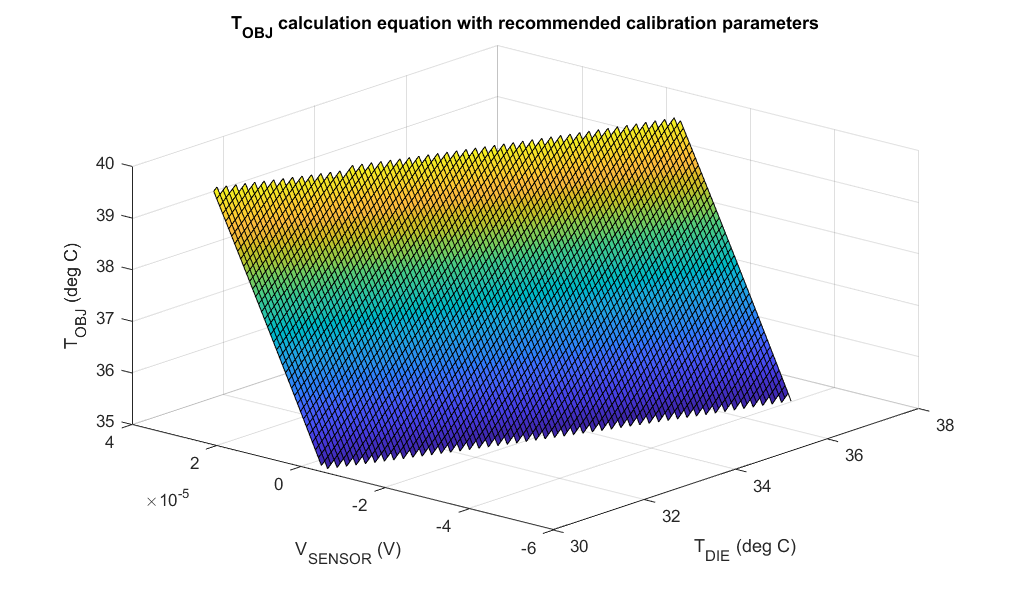
\includegraphics[width=14cm,height=7.5cm]{figs/RecommendedTempCurve.png}
   \caption{Plot of the the T\textsubscript{OBJ} equation with recommended calibration parameters over the operating temperature range of the Ear-Monitor}
   \label{fig:RecommendedTempCurve}
\end{figure}

This linear characteristic of the TMP006 in the operating temperature range of the Ear-Monitor can be used to simplify the T\textsubscript{OBJ} calculation method as described in Equations \ref{eq:TempCurve1} to \ref{eq:TempCurve4}. These bulky recommended equations can be replaced by a first degree polynomial formula for a flat plane as described by:
\begin{equation}
\label{eq:FlatPlane}
T_{OBJ}=P0+P1\cdot T_{DIE}+P2\cdot V_{SENSOR}
\end{equation}
Where $P0$, $P1$ and $P2$ are parameters to be determined by a calibration process that follows the trial stage.

\subsection{PPG signal processing}
The PPG signal is crucial to the calculation of heart rate, respiratory rate and SpO\textsubscript{2}. This signal is captured by the MAX30100 pulse oximeter. Some noise is present in the measured signal. The MAX30100 has on chip digital filters for 50Hz/60Hz interference and low-frequency ambient noise. Despite on-chip filtering, signal drift and high frequency noise still contaminate the signal. This causes the detection of false heart beat peaks and noisy SpO\textsubscript{2} calculations. An AC and DC extraction algorithm and low-pass filter is designed to prime the signal for further processing. Figure \ref{fig:PPG_Filtering} shows how the signal samples for the MAX30100 are processed.  $x_n$ is the PPG signal measured by the MAX30100 in the ear canal and $y_n$ is the processed signal.

\begin{figure}[H]
\centering
\graphicspath{{figs/}}
%\def\svgwidth{180pt}
\input{figs/PPG_Filtering.pdf_tex}
\caption{The raw PPG signal, $x_n$, is sent through AC and DC extraction and filtering functions}
\label{fig:PPG_Filtering}
\end{figure}

\subsubsection{AC and DC separation}
An algorithm is implemented to digitally separate the AC and DC components of the red and IR signals. Signal separation need to be done in real time and with the minimal computational overhead, because it is executed on the MCU. The following infinite impulse response (IIR) filter is used for AC extraction \citep{koblenski2015everyday}:
\begin{align}
\label{eq:AC_Extraction}
w_n= x_n  + \alpha\cdot w_{(n-1)}\\
y_n  = w_n  - w_{(n-1)}
\end{align}
Where $x_n$ is the raw ADC value from the MAX30100, $w_n$ is an intermediate value and $y_n$ is the filter output. This filter has a narrow stop band at the DC frequency when the scale factor,  $\alpha$, is close to 1. Scale factor $\alpha=0.7$ is chosen as it gives the best DC rejection while maintaining an acceptable response time. Figure \ref{fig:AC_Extraction} shows the PPG signal before and afted the C extraction function.

\begin{figure}[H]
   \centering
   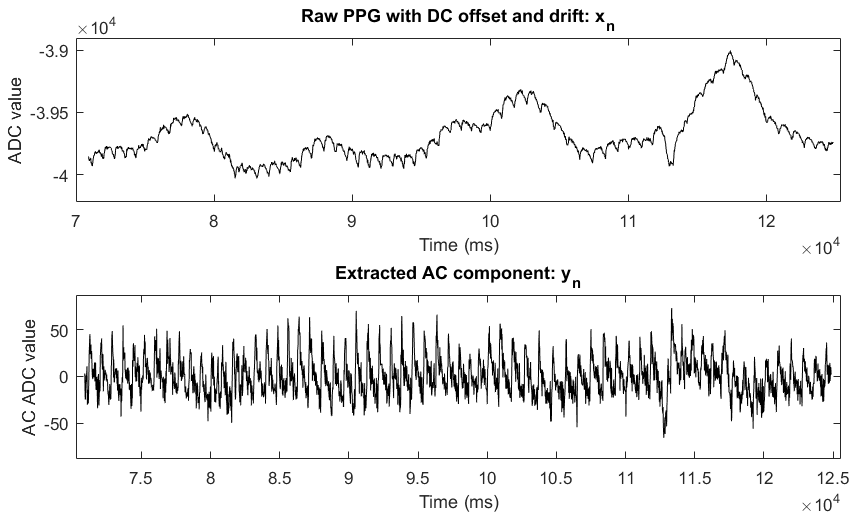
\includegraphics[width=12cm,height=7.5cm]{figs/AC_Extraction.png}
   \caption{(a) the raw IR signal contaminated by DC offset and drift and (b), the extracted AC component of the signal}
   \label{fig:AC_Extraction}
\end{figure}

The DC component of the signal is used during LED bias adjustment and SpO\textsubscript{2} calculations. To get the DC value, the AC value is subtracted from the raw signal. Alternative AC extraction methods tested were high-pass FIR filtering and moving average subtraction. These methods were rejected, because a high-pass FIR filter is to computationally intensive and moving average subtraction will attenuate frequencies close to DC as well.

\subsubsection{Low-pass filter}
The separated AC and DC component of the red and IR signals are passed through a third order IIR Butterworth filter. The coefficients were calculated with MATLAB for a cut-off frequency of 3 Hz. Equation \ref{eq:TransferFunc} is the transfer function H(z) of the filter.
\begin{equation}
\label{eq:TransferFunc}
H(z) = \frac{0.0048+0.0143z^{-1}+0.0143z^{-2}+0.0048z^{-3}}{1.0000-2.2501z^{-1}+1.7564z^{-2}-0.4683z^{-3}}
\end{equation}

Figure \ref{fig:PPG_Filter} shows the effect of the low-pass filter on the AC signal as extracted in the AC and DC separation function. 

\begin{figure}[H]
   \centering
   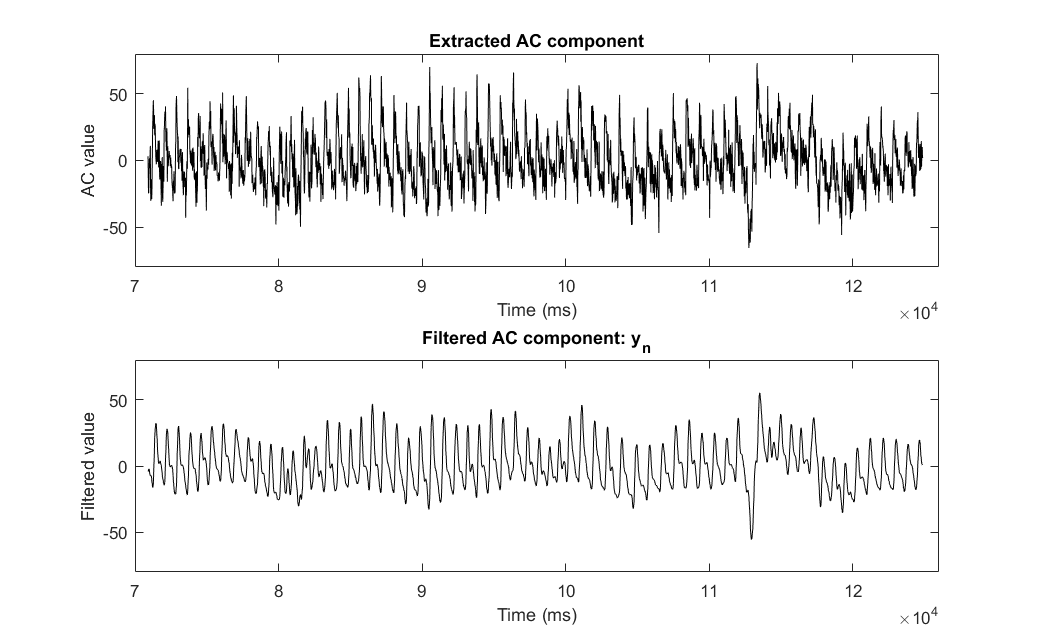
\includegraphics[width=12cm,height=7.5cm]{figs/PPG_Filter.png}
   \caption{(a) the AC component of the IR signal before filtering and (b), after filtering}
   \label{fig:PPG_Filter}
\end{figure}

\subsection{Beat Detection}
Heart beats appear as peaks on the inverted PPG signal. The IR PPG is chosen for beat detection, for IR light absorption by oxyhaemoglobin is higher than that of red light. Therefore, IR pulse peaks are more prominent, thus better suited for the detection of heart beats. A software algorithm is developed to detect these peaks in order to calculate average heart rate, breathing rate and SpO\textsubscript{2}. The algorithm takes as input the filtered IR PPG signal y\textsubscript{n}, and outputs a timeseries of the heart beats. Figure \ref{fig:PPG_SignalLabels} shows a plot of a PPG signal with characteristic features labelled.

\begin{figure}[H]
\centering
\graphicspath{{figs/}}
\input{figs/PPG_SignalLabels.pdf_tex}
\caption{Filtered AC component of PPG with important features labelled}
\label{fig:PPG_SignalLabels}
\end{figure}

This signal extract shows the challenges of the peak detection algorithm. The amplitude of the peaks varies significantly and local maxima which can trigger false positives are present. The intermediate peak in the descending part of the peak is the dicrotic notch, due to the aortic valve closing. Only true systolic peaks should be registered as a hear beat. The beat detection algorithm needs to be robust, computationally inexpensive and should not require any user-specific modifications. 

\medskip

These obstacles are overcome by a two-stage peak detection algorithm developed specifically for the Ear-Monitor's PPG. The algorithm builds on the work done by \cite{park2015wearable}, \cite{zong2003open} and \cite{elgendi2013systolic} as well as adding new elements like the ...

\medskip

Stage 1 is a morphological conversion in the form of a slope summing function (SSF). This method is also used by \cite{zong2003open}, \cite{park2015wearable} and \cite{elgendi2013systolic}. The SSF is defined piecewise according on its derivative, $\Delta y_n$,  as shown by Equation \ref{eq:SSF}. The aim of the SSF is to enhance the rising section of the pulse peak while suppressing the falling section.

\begin{equation}
\label{eq:SSF}
z_n = \sum\limits_{k=n-w}^n \Delta y_k, \quad \text{where} \quad \Delta y_k=
\begin{cases}
\Delta y_k, 	&\text{if } \Delta y_k \textless	0 \\
0, 				&\text{if } \Delta y_k \geq			0. 
\end{cases}
\end{equation}

The n\textsuperscript{th} SSF output value, $z_n$,  equals the sum of the previous $w$ filtered PPG slopes as defined by the conditions in Equation \ref{eq:SSF}. \cite{zong2003open} suggest choosing $w$ as the typical duration of the pulse up-slope, so a moving sum window of $w=10$ was selected. Figure \ref{fig:SSF} shows (a) the extracted  and filtered AC component and (b) the output of the SSF.

\begin{figure}[H]
   \centering
   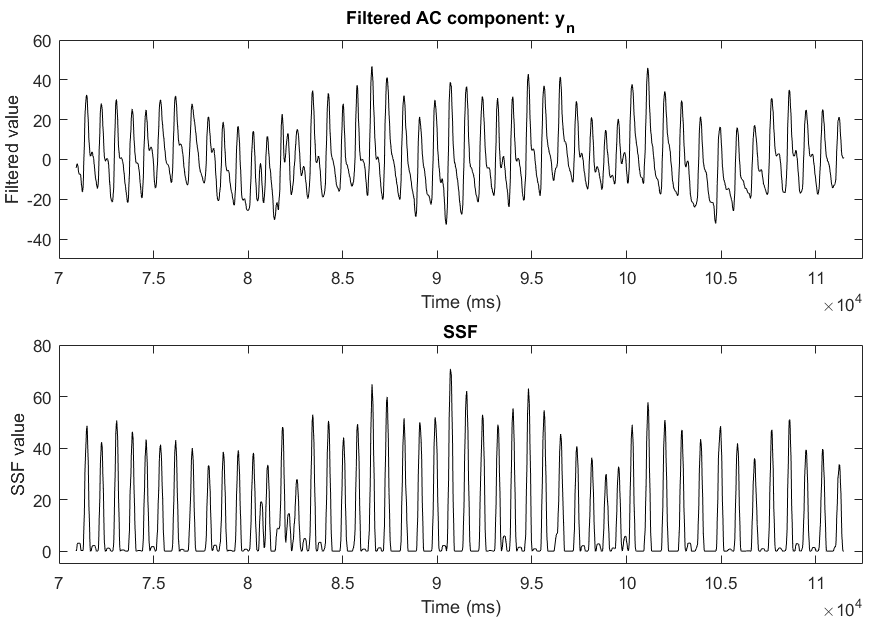
\includegraphics[width=12cm,height=7.5cm]{figs/SSF.png}
   \caption{(a) the AC component of the IR signal before filtering and (b), after filtering}
   \label{fig:SSF}
\end{figure}

Stage 2 of the beat detection function is a set of decision rules determine if a peak is present. Some of the rules were adapted form \cite{park2015wearable}. Their algorithm is applied to in-ear pulse waves, which is closer to a ballistocardiogram than a PPG. Therefore, the decision rules in this function are chosen specifically for the Ear-Monitor and determined through experimentation.

\medskip

Rule 1: Adaptive threshold. The adaptive threshold applied to this algorithm is related to the mean of the previous 3 detected SSF peak heights by Equation \ref{eq:Threshold}.

\begin{equation}
\label{eq:Threshold}
t=c\frac{\sum\nolimits_{k=0}^2 z_{n-k}}{3}
\end{equation}

Where $c$ is an experimentally determined scaling factor equal to 0.5. If the SSF signal amplitude rises above the threshold, a potential peak is awaited. \cite{zong2003open} uses a threshold equal to 60\% of the previous SSF peak amplitude, but this method proved to miss heartbeats if subsequent SSF maxima varies more that the threshold percentage. This problem is mitigated by basing the threshold on the previous three-peak average.

\medskip

Rule 2: Local maximum point. Following the crossing of the threshold, the algorithm monitors the SSF for a local maximum. This occurs at $SSF_{n-1}$ when: $SSF_{n-2} < SSF_{n-1} \ge SSF_n$.

\medskip

Rule 3: Waiting period
If a local maximum is detected, the time elapsed since the previous successfully detected beat is tested. If the time is less than a dynamic waiting period, the local maximum is rejected. The waiting period is set to be 70\% of the mean of the previous 10 beat periods.

\medskip

Only if all three rules apply to a SSF value, will it be registered as a peak. The time difference between the newly detected peak and the previous one is the heart beat period. Another element to the beat detection algorithm is the threshold reset. If no local maximal is detected abouve the threshold for longer than 2 times the mean of the previous 10 beat periods, the threshold is reset to 1. This is in case the amplitude of the SSF peaks drops below the threshold and no beats is registered to update the threshold to a lower value. Figure \ref{fig:BeatDetection} shows the example signal's SSF with detected beats. This example illustrates how the algorithm can successfully detect peaks of varying amplitude and using the threshold method and how the time delay prevent the triggering of a false peak.

\begin{figure}[H]
   \centering
   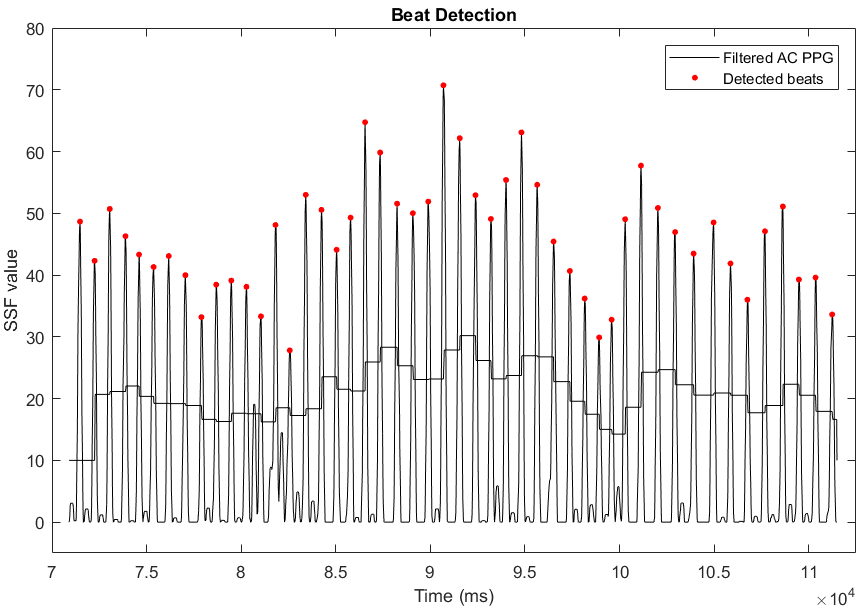
\includegraphics[width=12cm,height=7.5cm]{figs/BeatDetection.png}
   \caption{SSF with detected beats and threshold plotted.}
   \label{fig:BeatDetection}
\end{figure}

\subsubsection{Respiratory- and Heart Rate Calculation}
Respiration rate is determined by monitoring respiratory sinus arrhythmia (RSA), the frequency modulating respiratory related heart rate characteristic.

\subsection{SpO\textsubscript{2} Calculation}
The MAX30100 outputs digitals value representing the intensity of red and IR light reflected by the tissue. Due to the different absorption spectra of oxygenated and deoxygenated blood, these values can be used to determine the fraction of peripheral blood oxygen saturation. PC software is written to calculate the SpO2 and MCU software is written to control the sensor. 

\subsection{Current Balancing}
The ratio of ratios method, discussed in the literature review and shown in Equation \ref{eq:SatsRatio}, is used to calculate SpO2.

\begin{equation}
\label{eq:SatsRatio}
R = \frac{\left(\frac{AC}{DC}\right)\textsubscript{red}}{\left(\frac{AC}{DC}\right)\textsubscript{IR}}
\end{equation}

The motivation behind using this method is that it compensates for differences in DC reflection from person to person. For this to work, the difference between the red and IR DC values used in the equation needs to be as small as possible. The current to the red and IR LED of the MAX30100 are set to \SI{50}{\milli\ampere} upon start-up configuration. To compensate for the fact that IR light is reflected differently by the tissue than red light, a dynamic current balancing function is written.

\medskip

The MAX30100 has a programmable register that allows for the individual current adjustment of red and IR LED drivers. A negative feedback control system is implemented on the MCU to adjust the individual LED currents in order to lower the difference in reflection. A lower current equals a lower light intensity and subsequently, less reflection.

The function checks the difference in IR and red DC levels every second and adjusts the current to the LEDs until the difference are within an acceptable margin. Figure \ref{fig:CurrentBalancing} shows a plot of this process. The difference in reflection starts out at 15000, with both LED currents equal to \SI{50}{\milli\ampere}, and after five adjustments the difference is lowered to 1000, with the red LED current unchanged and the IR LED equal to \SI{33.9}{\milli\ampere}. As can be seen from Figure \ref{fig:CurrentBalancing}, the current adjustments happen in a stepwise fashion, with each step about 2700. Therefore, to avoid oscillations, the margin is set to 2000.

\begin{figure}[H]
   \centering
   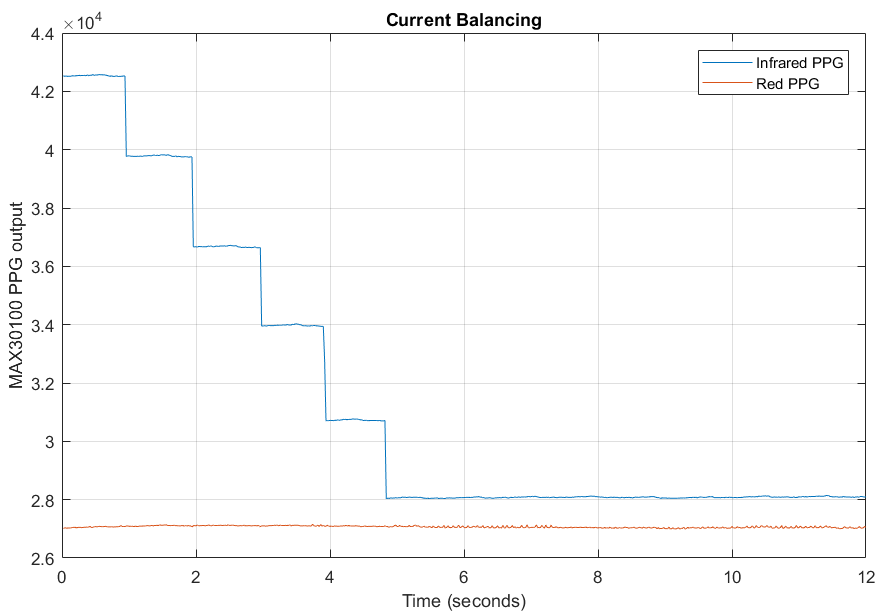
\includegraphics[width=12cm,height=7.5cm]{figs/CurrentBalancing.png}
   \caption{Plot showing the effect of the current balancing function implemented on the MAX30100 lowering the difference in detected light between red and IR LED by adjusting the current to the IR LED.}
   \label{fig:CurrentBalancing}
\end{figure}

\subsection{Moving average SpO\textsubscript{2}}
SpO\textsubscript{2} calculation is done by the PC interface software. The filtered AC and DC components of the IR and red PPG signals, as calculated in the PPG signal processing section, are used in the ratio of ratios method. $R$ is calculated using the mean of the absolute AC and DC values of the previous 12 heartbeats. These values are updated each time new PPG data is available.

\medskip

The relationship between $R$ and SpO\textsubscript{2} is unique for different devices and measurement locations. Calibration is needed to find the relation for die Ear-Monitor. The relationship used in literature \citep{ti2012application} was adjusted though a calibration process to achieve a desirable level of accuracy. Equation \ref{eq:Sats} shows the relationship used by the Ear-Monitor to calculate SpO.\textsubscript{2}.

\begin{equation}
\label{eq:Sats}
111.2-(25\cdot R)
\end{equation}

$R$ and SpO\textsubscript{2} are calculated on every heartbeat using the moving data window of the previous 12 heartbeats.

\subsection{PC Interface}
A graphical user interface is written in Processing to display the measurements on the computer screen and allow the user to set alarms and save the data. The interface receives variables from the various functions discussed. It displays these variables along with a series of real-time graphs and has the option to save the measured Ear-Monitor data in a .csv file for later reference or analysis. Figure \ref{fig:GUI} shown 

\begin{figure}[H]
\centering
\graphicspath{{figs/}}
%\def\svgwidth{180pt}
\input{figs/GUI.pdf_tex}
\caption{Ear-Monitor user interface with (a) the SSF with detected beats, (b) the AC components of the red and IR PPGs, (c) respiration illustrated in plotting the heart beat period, (d) temperature, (e) data written to .cvs files and (f) alarm conditions}
\label{fig:GUI}
\end{figure}
\chapter{Trial Period}
\label{chp:Trial Period}
A trial is conducted during which the Ear-Monitor is tested on a group of 16 healthy, adult volunteers. The trial's goal is twofold: firstly to to calibrate the temperature and SpO\textsubscript{2} algorithms and secondly to evaluate the accuracy of the Ear-Monitor's measurements. This chapter describes the trial environment and the method used to collect data for calibration and evaluation. Ethical approval is obtained for this trial form the Health Research Ethics Committee of Stellenbosch University, under the reference number M16/09/038 (proof of approval included in Appendix X).

\section{Participant Selection}
Participants for the study are invited via a recruitment email sent to students and staff at the faculty building. Inclusion criteria are physical health, ages from 18 to 60 years and volunteers of any gender or race. Exclusion criteria are small ear canal size, ear abnormalities or injuries and general health issues. If the individual's ear canal is smaller than 5 mm diameter the Ear-Monitor's probe will not fit. This also applies to ear abnormalities or injuries that will prevent the use of an ear probe, for example an abnormal sharp bend in the ear canal or an inflamed or infected ear canal due to i.e. otitis externa (swimmers ear). Individuals with self diagnosed illness that will cause them risk if they participate, are also excluded. Potential participants are screened through a pre-test physical examination to determine if they meet all the criteria. Table \ref{tab:Participants} gives a demographic summary of the participants that are selected for the trail.

\begin{table}[H]
\caption{Demographic summary of participants}
\label{tab:Participants}
\renewcommand{\arraystretch}{1.1}	%Wat doen hierdie?
\centering
\begin{tabular}{P{3cm} P{3cm} P{3cm}} 
\hline
						& 	n			&			Average age\\ 
\hline
Male					&	13			&			24.5 $\pm$ 0.7\\
Female  				&	3			&			23.3 $\pm$ 0.3\\
Total  					&	16			&			24.3 $\pm$ 0.6\\
\hline
\end{tabular}
\end{table}

\section{Benchmark Validation}
Evaluation is done for all four medical signs measure by the Ear-Monitor, namely core temperature, heart rate, respiratory rate and SpO\textsubscript{2}. Evaluation entails comparing the medical sign measurements made by the Ear-Monitor to measurements made, in the same conditions, by industry standard medical devices, referred to as benchmark devices. The measurements made by benchmark device is referred to as benchmark measurements. In this trial, a device that conforms to the EC requirements is seen as a benchmark device. The CE mark is sign that the benchmark device complies with the ISO 13485 standard for medical devices, which requires industry standard accurate measurements.

\medskip

Three benchmark devices, shown in Figure \ref{fig:Benchmark}, are selected to provide the various benchmark measurements. A concise technical overview is given of each.

\begin{figure}[H]
\centering
\graphicspath{{figs/}}
\input{figs/Benchmark.pdf_tex}
\caption{Benchmark devices: (a) Nexus-10, (b) SureSigns VM1 and (c) EM 100-A}
\label{fig:Benchmark}
\end{figure}

The Nexus-10 physiological monitoring platform is selected to provide benchmark heart rate and respiratory rate measurements. The Nexus-10 is a data acquisition device with a 24-bit analogue to digital converter and a accuracy of $\pm$2\% according to the manufacturer. It has a blood volume sensor, which measures a PPG signal from the fingertip at a sampling rate of 128 Hz. This PPG signal is used to provide the benchmark heart rate measurement. It also has an elastic chest strap to measure respiratory rate. The movement of the chest during the respiratory cycle is converted to a voltage signal and digitalized at a sampling rate of 32 Hz. This signal is used to provide the benchmark respiratory rate measurement. It uses a Bluetooth connection to send data to a computer. The BioTrace+ software package is used to display the recorded data in real time as well as store the data for later processing.

\medskip

The SureSigns VM1 patient monitor from Philips is selected to provide benchmark SpO\textsubscript{2} measurements. The SureSigns VM1 uses a pulse oximeter attached to the fingertip to measure SpO\textsubscript{2}. Data is logged on the device's screen and updated at 1 Hz and stored on a computer for later processing. The device is recommended for use by healthcare professionals, emphasizing its accuracy and reliability.

\medskip

The ET-100A infrared ear thermometer is selected to provide the benchmark tympanic ear temperature measurements. The ET-100A complies with the EN12470-5:2003 standard for clinical thermometers, therefore satisfies a accuracy of $\pm$\SI{0.2}{\celsius} over the range of \SI{35.5}{\celsius} to \SI{42}{\celsius}. Its measurements are displayed on the device's screen and data is entered and stored on a computer for later processing.


\section{Method}
Data is recorded from one participant at a time. A recording session involves collecting four benchmark- and four Ear-Monitor medical sign measurements simultaneously from one participant. Each recoding session lasts for 2 minutes and is conducted twice per participant to ensure repeatability. Figure \ref{fig:SetUp} shows a diagram of how all the devices are connected to the participant and which measurements are made by each.

\begin{figure}[H]
\centering
\graphicspath{{figs/}}
\input{figs/SetUp.pdf_tex}
\caption{Diagram showing how devices are connected to the participant during the recording session}
\label{fig:SetUp}
\end{figure}

The recording session can be summed up as follows:

\begin{itemize}
\item The trial environment is set up before the participant arrives. Equipment is disinfected and connected to the computer, ready for data capture. 
\item The participant arrives and is briefed about the procedure and signs an informed consent form. The participant is also asked to clean his/her ear with surgical spirits.
\item The participant is seated stationary in front of a table containing all the equipment. Sensors are placed on the participant as shown in Figure \ref{fig:SetUp}. Three tympanic temperature benchmark measurements are taken from the participant with the ET 100-A.
\item The recording session starts. The participant sits still the entire time and breaths normally for the first 60 seconds, after which the participant is asked to breath at 15 breaths per minute by following breathing metronome for another 60 seconds.
\item After 60 of controlled breathing (120 seconds recording time in total) the recording session is concluded. Three more temperature benchmark measurements are taken with the ET 100-A.
\item Data from the Ear-Monitor and benchmark devices is stored on a computer in .cvs format for later processing and analysis.
\end{itemize}

The breathing exercise is included due to the uncertainty that the RSA will be detectable during normal breathing. During prototyping it was more visible in beeper forced breathing. Therefore, if it is not detectable in normal breathing, the controlled breathing data can still be analysed to produce some results. 

\medskip

Figure \ref{fig:TrialPhoto} shows an image of one of the participants during a data recording session. The labelled equipment is (a) the computer with the Ear-Monitor user interface, (b) the Ear-Monitor on the participant with the red light of the MAX30100 visible through the tragus. (c) is the SureSigns VM1 and (d) its SpO\textsubscript{2} finger clip. (e) is the Nexus-10 and (f) its blood volume sensor finger clip and (g) its chest strap for measuring respiration. The ET 100-A tympanic thermometer is labelled (h).

\begin{figure}[H]
\centering
\graphicspath{{figs/}}
\input{figs/TrialPhoto.pdf_tex}
\caption{Recording session set-up with participant}
\label{fig:TrialPhoto}
\end{figure}



%==== Appendices ====================================================
\appendix
\appendixpage\relax

%\chapter{Discrete Element Method Theory}
\label{chp:DEM-Theory}

\section{Ball elements}
\label{sec:Ball-elems}

\begin{figure}
   \centering
   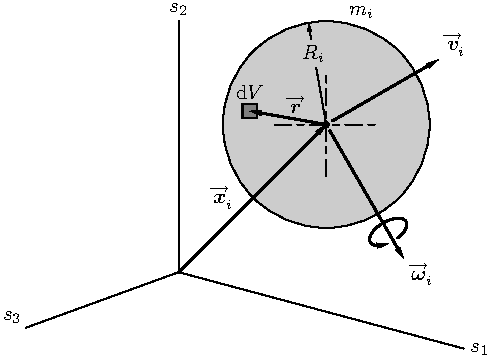
\includegraphics{figs/DEM-Def-Ball}
   \caption{Ball Element Parameters}
   \label{fig:BallDef}
\end{figure}


\subsection{Ball mass and inertia parameters}

Consider a volume element $\mathrm{d}V$ with respect to a static base $S$ of
an arbitrary solid body with  density $\rho$. The mass of the body is
obtained by integrating over the volume of the body,
\begin{equation}
    m = \int\limits_{\mathrm{body}} \rho\, \mathrm{d}V
    \label{eq:BMass-dif}
\end{equation}

In figure~\ref{fig:BallDef}, a ball with radius $R_{i}$ and uniform density
$\rho_i$ is depicted. The mass of the ball is after integration of
equation~\eqref{eq:BMass-dif}
\begin{equation}
    m_i = \tfrac{4}{3} \pi \rho_i\, R_i^3 .
    \label{eq:BMass}
\end{equation}


%----------------------------------------------------------------------------
\endinput

%\include{contents/App-2}
%\include{contents/App-3}

%==== Bibliography acro's & Index ===================================
\backmatter

\bibliography{backmatter/USbib-sample}
%\bibliographystyle{srtnat}%%<<<<<<<<<<<<<<<<<<<<<<<<<<<<<<<<<<<<<<<<<<<<<<<<<<<<<<<<<<<<<<<<<<<<<<<<<<<<<<<<<<<<<<<<<<<<<<<<<Vancouver
\end{document}
